%================================================================%
%======  Modelo de Monografia ( UFOP - DECOM) ===================%
% Proposta de texto em conformidade com normas da ABNT ----------%
% implementadas pelo projeto abntex2, que pode ser acessado pela %
% página  http://abntex2.googlecode.com/  -----------------------%
%================================================================%
\documentclass[12pt, % tamanho da fonte
   %openright,	     % capítulos começam em página ímpar
	oneside,		  % twoside para impressão em frente e verso.  
	a4paper,			% tamanho do papel. 
	english,			% Idioma adicional para hifenização
    brazil,				% Idioma principal 
    sumario=tradicional % Comente para o sumário ser conforme a opção padrão recomendada pela ABNT NBR 6027:2012.
	]{abntex2}
	
%------------------------------------------------------------
%------------    Estrutura do texto   -----------------------      

% Pacotes Básicos:
\usepackage[T1]{fontenc}		% Seleção de códigos de fonte.
\usepackage[utf8]{inputenc}		% Codificação do documento (conversão automática dos acentos)
\usepackage{lastpage}		    % Usado pela Ficha catalográfica
\usepackage{indentfirst}		
\usepackage{color}				% Controle das cores
\usepackage{graphicx}			% Inclusão de gráficos
\usepackage{tabularx}
\usepackage{microtype} 		  	% Melhorias da justificação
\usepackage{pdfpages}           %inserir páginas em PDF
% Pacotes Extras:
\usepackage{amsmath,amsthm}     % Símbolos Matemáticos
\usepackage[portuguese, ruled, linesnumbered,commentsnumbered, algo2e, vlined, lined, boxed, algochapter]{algorithm2e} % Algoritmos 
\usepackage{hyperref}      % Criação de links.

% Escolha da formatação das referências Bibliográficas: 
\usepackage[alf,abnt-etal-list=0,abnt-etal-cite=3]{abntex2cite}	% Citações padrão ABNT  (AUTOR, ANO)
\usepackage{etoolbox}
%\usepackage[num]{abntex2cite}  % Citações numéricas (1)
%\citebrackets[] % Usar este comando para a citação numérica aparecer com [].

% Numeração das Figuras e Tabelas
\counterwithin{figure}{chapter}
\counterwithin{table}{chapter}

% Defininção de Cores:
\definecolor{blue}{RGB}{25,25,112}
\makeatletter % informações do PDF
\hypersetup{
    %pagebackref= false,
	pdftitle={\@title}, 
	pdfauthor={\@author},
    %pdfsubject={\imprimirpreambulo},
	pdfcreator={LaTeX with abnTeX2},
	pdfkeywords={abnt}{latex}{abntex}{abntex2}{trabalho acadêmico}, 
	colorlinks=true,    % false: boxed links; true: colored links
    linkcolor=blue,     % color of internal links
    citecolor=blue,     % color of links to bibliography
    filecolor=magenta, 	% color of file links
	urlcolor=blue,
	bookmarksdepth=4
}
\makeatother

% -------------------------------------------- 
% Espaçamentos entre linhas e parágrafos 
\setlength{\parindent}{1.3cm} % O tamanho do parágrafo

% Controle do espaçamento entre um parágrafo e outro:
\setlength{\parskip}{0.2cm}  % tente também \onelineskip

% Definição de ambientes matemáticos em português 
\newtheorem{teorema}{Teorema}[chapter]
\newtheorem{axioma}{Axioma}[chapter]
\newtheorem{corolario}{Corolário}[chapter]
\newtheorem{lema}{Lema}[chapter]
\newtheorem{proposicao}{Proposição}[chapter]
\newtheorem{definicao}{Definição}[chapter]
\newtheorem{exemplo}{Exemplo}[chapter]
\newtheorem{observacao}{Observação}[chapter]

% Novos Comandos
\usepackage{tgtermes}
\renewcommand{\ABNTEXchapterfont}{\rmfamily\bfseries}

% Variáveis adicionais
\providecommand{\imprimirautorcite}{}
\newcommand{\autorcite}[1]{\renewcommand{\imprimirautorcite}{#1}} 
\providecommand{\imprimirsubtitulo}{}
\newcommand{\subtitulo}[1]{\renewcommand{\imprimirsubtitulo}{#1}} 
\providecommand{\imprimirsigla}{}
\newcommand{\sigla}[1]{\renewcommand{\imprimirsigla}{#1}}
\providecommand{\imprimiruf}{}
\newcommand{\uf}[1]{\renewcommand{\imprimiruf}{#1}}
\providecommand{\imprimircurso}{}
\newcommand{\curso}[1]{\renewcommand{\imprimircurso}{#1}}
\providecommand{\imprimirinstituto}{}
\newcommand{\instituto}[1]{\renewcommand{\imprimirinstituto}{#1}}
\providecommand{\imprimirdepartamento}{}
\newcommand{\departamento}[1]{\renewcommand{\imprimirdepartamento}{#1}}
\providecommand{\imprimirano}{}
\newcommand{\ano}[1]{\renewcommand{\imprimirano}{#1}}
\providecommand{\imprimirgrau}{}
\newcommand{\grau}[1]{\renewcommand{\imprimirgrau}{#1}}
\providecommand{\imprimirexaminadorum}{}
\newcommand{\examinadorum}[1]{
    \renewcommand{\imprimirexaminadorum}{#1}}
\providecommand{\imprimirexaminadordois}{}
\newcommand{\examinadordois}[1]{
    \renewcommand{\imprimirexaminadordois}{#1}}
\providecommand{\imprimirexaminadortres}{}
\newcommand{\examinadortres}[1]{
    \renewcommand{\imprimirexaminadortres}{#1}}
\providecommand{\imprimirexaminadorquatro}{}
\newcommand{\examinadorquatro}[1]{
    \renewcommand{\imprimirexaminadorquatro}{#1}}
\providecommand{\imprimirttorientador}{}
\newcommand{\ttorientador}[1]{
    \renewcommand{\imprimirttorientador}{#1}} 
\providecommand{\imprimirttcoorientador}{}
\newcommand{\ttcoorientador}[1]{
    \renewcommand{\imprimirttcoorientador}{#1}}
\providecommand{\imprimirttexaminadorum}{}
\newcommand{\ttexaminadorum}[1]{
    \renewcommand{\imprimirttexaminadorum}{#1}}
\providecommand{\imprimirttexaminadordois}{}
\newcommand{\ttexaminadordois}[1]{\renewcommand{
        \imprimirttexaminadordois}{#1}}
\providecommand{\imprimirttexaminadortres}{}
\newcommand{\ttexaminadortres}[1]{
    \renewcommand{\imprimirttexaminadortres}{#1}}
\providecommand{\imprimirttexaminadorquatro}{}
\newcommand{\ttexaminadorquatro}[1]{
    \renewcommand{\imprimirttexaminadorquatro}{#1}}
		
%----------------------------------------------------
\renewcommand{\imprimircapa}{ % Capa 
\begin{capa}
        \begin{center}
                \begin{DoubleSpace}
                
\includegraphics[scale = 0.2]{Figuras/Uni7.png} \\
                \MakeUppercase{\imprimirinstituicao } \\
                 \MakeUppercase{\imprimirinstituto } \\
                \end{DoubleSpace}
                \vspace{5cm}
				\MakeUppercase{\imprimirautor}  \\
                \imprimirorientadorRotulo ~\imprimirorientador \\
                \imprimircoorientadorRotulo ~\imprimircoorientador \\
                        				
				\vspace{5cm}
             \textbf{{\large\MakeUppercase{\imprimirtitulo}}} \\
			 \textbf{{\large \MakeUppercase{\imprimirsubtitulo}}} \\
				\vfill
        {\large{\imprimirlocal, ~\imprimiruf \\ \imprimirano  }}
        \end{center}
\end{capa}   
} % Capa



%----------------------------------------------------
\renewcommand{\imprimirfolhaderosto}{% folha de rosto
       \begin{center}
                \MakeUppercase{\imprimirinstituicao } \\
                 \MakeUppercase{\imprimirinstituto } \\
                \MakeUppercase{\imprimirdepartamento} \\
                
                \vspace{4cm}
				\MakeUppercase{\imprimirautor}  \\
				\vspace{2cm}
			    \begin{DoubleSpace}
                \MakeUppercase{\textbf{\imprimirtitulo} } \\
                \MakeUppercase{\textbf{\imprimirsubtitulo}} \\
                \end{DoubleSpace} 
      \end{center}
    \vfill 
    \begin{flushright} 
    \parbox{0.6\linewidth}{
		\imprimirtipotrabalho~ apresentada ao Curso de \imprimircurso~ da \imprimirinstituicao~ como parte dos
		requisitos necessários para a obtenção do grau de \imprimirgrau. \\ \\
		\textbf{\imprimirorientadorRotulo}~\imprimirorientador \\
		\textbf{\imprimircoorientadorRotulo}~\imprimircoorientador}
   \end{flushright} 
		\vfill
   \begin{center}
   {\large{\imprimirlocal, ~ \imprimiruf \\
   \imprimirano} }
   \end{center} }  % folha de rosto

%----------------------------------------------------


 % Estrutura do documento e pacotes usados. Outros pacotes (packages) devem ser  adicionados ao arquivo structure.tex. 


% -- Informações para Capa e Folha de Rosto: ---------------
\titulo{Desenvolvimento de Estação Meteorológica padrão EMS-3 com a plataforma Arduino para Aeroportos Regionais } 
\subtitulo{}
\autor{Jedson Cid Nascimento de Brito} \autorcite{Aluno, Nome}
\local{Fortaleza} \uf{CE}
\data{15 de Setembro de 2020} \ano{2020}
\orientador{Prof. Dr. Alex Lacerda Ramos}  % Nome do orientador. Caso seja uma orientadora use o comando ∖orientador[Orientadora:]{Nome}
\ttorientador{Instituto Federal do Ceará - Campus Morada Nova} % Instituição do orientador
\ttcoorientador{Universidade 7 De Setembro} % Instituição do Coorientador
\instituicao{Centro Universitário 7 De Setembro UNI7} \sigla{UNI7}
\instituto{Especialização em Desenvolvimento de Sistemas para Dispositivos Móveis}
\departamento{Departamento de Computação}
\curso{Especialização em Desenvolvimento de Sistemas para Dispositivos Móveis}	
\tipotrabalho{Monografia} % Monografia (Monografia II)
\grau{Pós-Graduação}

%------Nomes dos membros da banca.  
\examinadorum{Prof. Dr. Danilo Reis de Vasconcelos}
\ttexaminadorum{Instituto Federal do Ceará - Campus Morada Nova}
\examinadordois{Prof. MSc André Jackson Gomes Bessa}
\ttexaminadordois{Universidade 7 De Setembro - UNI7}
%\examinadortres{Prof. Dr. Membro da Banca  3} 
\ttexaminadortres{Universidade Federal de ... - UFXX}
%\examinadorquatro{Prof. Dr. Membro da Banca  4}
\ttexaminadorquatro{Universidade Federal de ... - UFXX}

% ------------------------------------------------------
\makeindex   

\begin{document} % Início do documento

\frenchspacing  % Retira espaço obsoleto entre as frases.

% ----------------------------------------------------------
% -- Elementos Pré-Textuais: -------------------------------
\pagenumbering{roman}

\imprimircapa  % Capa
\imprimirfolhaderosto % Folha de rosto
%% ---------------------------------------------------------------
% ----------------  Ficha Catalográfica  -------------------------
% ---------------------------------------------------------------
% Modelo de ficha catalográfica. Você deverá substituir esta
% folha na versão final da monografia por um pdf fornecido pela 
% biblioteca. Salve o modelo oficial como ficha_catalografica.pdf
% e use o comando abaixo para inseri-lo na versão final do texto.

%\begin{fichacatalografica}
%    \includepdf{ficha_catalografica.pdf}
%\end{fichacatalografica}



%% Modelo de Como fazer a Ficha Catalográfica:

\begin{fichacatalografica}
	\sffamily
	\vspace*{\fill}					% Posição vertical
	\begin{center}					% Minipage Centralizado
	\fbox{\begin{minipage}[c][8cm]{14cm}		% Largura
	\small
	\imprimirautorcite.
	%Sobrenome, Nome do autor
	
	\hspace{0.5cm}  \\
	\imprimirtitulo  / \imprimirautor. --, \imprimirano-
	
	\hspace{0.5cm} \pageref{LastPage} p. 1 :il. (colors; grafs; tabs).\\
	
	\hspace{0.5cm} \imprimirorientadorRotulo~\imprimirorientador\\
	
	\hspace{0.5cm}
	\parbox[t]{\textwidth}{\imprimirtipotrabalho~--~\imprimirinstituicao, ~ \\
	\imprimirinstituto, ~\imprimirdepartamento,~\imprimirano.}\\
	
	\hspace{0.5cm} % Palavras-chave do trabalho
		1. Palavra-chave 1.
		2. Palavra-chave 2.
		2. Palavra-chave 3.
		3. Palavra-chave 4.
		4. Palavra-chave 5.
		I. \imprimirorientador.
		II. \imprimirinstituicao.
		III. \imprimirtitulo  			
	\end{minipage} }
	\end{center}
\end{fichacatalografica}



%\begin{errata}

\noindent AUTOR, \textbf{\imprimirtitulo} \imprimirsubtitulo. nº de páginas. \imprimirtipotrabalho - 
\imprimirdepartamento, \imprimirinstituicao, \imprimirlocal, \imprimirano.

\begin{table}[!ht]
\centering
\begin{tabular}{|c|c|c|c|} \hline
\textbf{Página} & \textbf{Linha} & \textbf{Onde se lê} & \textbf{Leia-se} \\ \hline
16 & 10 & &  \\ \hline
\end{tabular}
\end{table}


Este elemento pré-textual é opcional e deve ser inserido no texto, geralmente após o trabalho já ter sido impresso, após a folha de rosto. Deve conter a referência do trabalho e o texto da errata com a indicação da página a linha \cite{NBR14724:2011}.

\end{errata}
% ---------------------------------------------------------------
% ----------------  Folha de aprovação  -------------------------
% ---------------------------------------------------------------
% Modelo de Folha de aprovação. Você deverá substituir esta folha na versão final da monografia por um pdf fornecido pelo colegiado do seu curso. Salve o modelo oficial como 
% folhadeaprovacao_final.pdf e use o comando abaixo para inseri-lo na versão final do texto. 
% A versão abaixo foi feita seguindo as normas ABNT NBR 14724:2011 em vigor.

%\begin{fichacatalografica}
%    \includepdf{folhadeaprovacao_final.pdf}
%\end{fichacatalografica} Esta folha será 


\begin{folhadeaprovacao}


\begin{center}
     {\large \imprimirautor}\\
       	\vspace{2cm}	
    \begin{DoubleSpace}    
    {\large \textbf{\MakeUppercase{\imprimirtitulo}}} \\
    {\large \textbf{\MakeUppercase{\imprimirsubtitulo}}}
    \end{DoubleSpace}
		\vspace{1cm}
        
\end{center}		


\begin{flushright} 
    \parbox{0.6\linewidth}{
		\imprimirtipotrabalho~ apresentada ao Curso de \imprimircurso~ da \imprimirinstituicao~ como parte dos
		requisitos necessários para a obtenção do grau em \imprimirgrau.\\}
   \end{flushright} 

\noindent Aprovada em \imprimirlocal,~ \imprimirdata. 
\begin{center}
\vfill
       \rule{10cm}{.1pt} \\
       {\imprimirorientador} \\ {\imprimirttorientador} \\
			 Orientador 
       \vfill
			 \ifdefvoid{\imprimircoorientador}{}{
       \rule{10cm}{.1pt} \\
       \imprimircoorientador \\ \imprimirttcoorientador \\ Coorientador }
			 \vfill
       \rule{10cm}{.1pt} \\
       {\imprimirexaminadorum} \\ {\imprimirttexaminadorum} \\ Examinador
        \vfill
        \ifdefvoid{\imprimirexaminadordois}{}{
        \rule{10cm}{.1pt} \\
        \imprimirexaminadordois \\ \imprimirttexaminadordois \\ Examinador}
				\vfill
        \ifdefvoid{\imprimirexaminadortres}{}{
        \rule{10cm}{.1pt} \\
        \imprimirexaminadortres \\ \imprimirttexaminadortres \\ Examinador}
				\vfill
        \ifdefvoid{\imprimirexaminadorquatro}{}{
        \rule{10cm}{.1pt} \\
        \imprimirexaminadorquatro \\ \imprimirttexaminadorquatro \\ Examinador}
\end{center}
  
\end{folhadeaprovacao}
% --- 
%\begin{dedicatoria}
   \vspace*{\fill}
   \centering
   \noindent
   \textit{ Espaço para prestar uma homenagem ou dedicar o trabalho a alguém.} 
	 \vspace*{\fill}
\end{dedicatoria}
%\begin{agradecimentos}

Espaço para agradecer às pessoas e/ou instituições que contribuíram de forma relevante à elaboração do trabalho.

\end{agradecimentos}

%\begin{epigrafe}
    \vspace*{\fill}
    
	\begin{flushright}
   Alguma citação importante para a construção do trabalho. A fonte deve ser indicada e também deve constar na lista de referências bibliográficas.
	\end{flushright}
    
\end{epigrafe}
%--------------------------------------------------------------------------
%--------------------- Resumo em Português --------------------------------
%--------------------------------------------------------------------------

\setlength{\absparsep}{18pt} % ajusta o espaçamento dos parágrafos do resumo
\begin{resumo}
As condições meteorológicas como vento, teto e visibilidade contribuem significativamente para os acidentes e incidentes aeronáuticos. Em razão disso, é muito importante que locais como aeroportos tenham suas próprias estações meteorológicas. No entanto, devido ao alto custo operacional desse tipo de equipamento especialmente para aeroportos regionais, poucos são os aeroportos que disponibilizam dados meteorológicos em tempo real. Diante desse cenário, esse trabalho propõe o desenvolvimento de um sistema de coleta de dados de meteorologia de baixo custo utilizando a plataforma arduino, aplicando o conceito de internet das coisas para disponibilizar os dados através da plataforma de nuvem ThingSpeak. Foi comparado dados coletados no protótipo elaborado com dados da plataforma REDEMET através de teste estatístico de comparação da média das variáveis meteorológicas e verificou que as médias das amostras são diferentes. 


 \vspace{\onelineskip}
 \noindent
 \textbf{Palavras-chave}: 1. Estação Meteorológica. 2. Arduino. 3.ThingSpeak. 4. Sensores Meteológicos 5.IOT.

%--------------------------------------------------------------------------As palavras-chave devem estar separadas por ponto e finalizadas também por ponto. Devem ser escolhidos termos  que descrevem o conteúdo do trabalho.
\end{resumo}

%--------------------------------------------------------------------------
%--------------------- Resumo em Inglês --------------------------------
%--------------------------------------------------------------------------
\begin{resumo}[Abstract]
 \begin{otherlanguage*}{english}
   Meteorological conditions such as wind, roof and visibility contribute significantly to aeronautical accidents and incidents. As a result, it is very important places like airports have their own weather stations. However, due to the high operational cost of this type of equipment, especially for regional airports, few airports provide real-time meteorological information. In this context, this work proposes to develop a low-cost meteorology data collect system using the arduino platform, applying the concept of internet of things(iot) to make data available through the cloud platform ThingSpeak. It was compared data collected in the prototype elaborated with data from the REDEMET platform through statistical test to compare the mean of the meteorological variables and found that the means of the samples are different.


   \vspace{\onelineskip}
   \noindent 
   \textbf{Keywords}: 1. Meteorological stations. 2. Arduino. 3.ThingSpeak. 4. Weather sensors 5. IOT.
 \end{otherlanguage*}
\end{resumo} % (Abstract no mesmo arquivo)

% As listas abaixo são opcionais. Caso o trabalho não possua alguma(s) dela(s) basta comentar os seus respectivos comandos.

% Lista de Figuras. 
\pdfbookmark[0]{\listfigurename}{lof}
\listoffigures*   
\cleardoublepage
% lista de Tabelas
\pdfbookmark[0]{\listtablename}{lot}
\listoftables*  
\cleardoublepage
% Lista de Algoritmos
%\pdfbookmark[0]{\listalgorithmcfname}{lof}
%\listofalgorithmes   
%\cleardoublepage

% Lista de Siglas e Símbolos. Estas listas são criadas manualmente e seus arquivos estão na pasta PreTextuais.
% ---------------------------------------------------
% ------ Lista de abreviaturas e siglas -------------
% ---------------------------------------------------
\begin{siglas}
  \item[DECEA] Departamento de Controle do Espaço Aéreo
  \item[EMA] Estação Meteorologica de Altitude
  \item[EMS] Estação Meteorológicas de Superfícies
  \item[FAB] Força Aérea Brasileira
  \item[ICA] Instruções do Comando da Aeronáutica
  \item[IDE] Ferramenta Integrada de Desenvolvimento
  \item[IOT] Internet das Coisas
  \item[INMET] Instituto Nacional de Meteorologia
  \item[OACI] Organização da Aviação Civil Internacional.
  \item[OMM] Organização da Meteorologia Mundial
  \item[REM] Rede de estalções meterológicas
  \item[REDEMET] Rede de Meteorologia do Comando da Aeronáutica
  
  
  

 
  
  
\end{siglas}
%% ---------------------------------------------------
% ----------- Lista de símbolos ---------------------
% ---------------------------------------------------

\begin{simbolos}
  \item[$ \V $] Volts
  \item[$ \ma $] Miliampere 
  \item[$ \C $] Celsius
  \item[$ \kt $] Nós
  \item[$ \hPa $] Hectopascal
\end{simbolos}

% Sumário:
\pdfbookmark[0]{\contentsname}{toc}
\tableofcontents*
\cleardoublepage

%% ------------- Capítulos ----------------------%%
\pagenumbering{arabic} \setcounter{page}{1}
\textual 
\chapter{Introdução} \label{Introducao}

O conhecimento de dados meteorológicos precisos e atuais são de suma importância para o planejamento de voos. Fenômenos de meteorologia adversos podem interferir nas atividades aeronáuticas de diversas formas suspendendo operações gerando cancelamentos, atrasos de voos \cite{costa2008meteorologia}. Nos últimos anos, a evolução tecnológica aprimorou várias ferramentas usadas para obtenção de dados do estado atmosférico, podemos destacar: sensores meteorológicos, imagens de satélite e radares. Apesar das suas diferenças, na forma de uso, todas convergem para o mesmo fim: monitorar e alertar sobre fenômenos climáticos, auxiliado na tomada de decisões.

Uma das estruturas da aviação que tem uma alta necessidade de possuir informações meteorológicas são os aeroportos, pois, estão vulneráveis a riscos resultantes da mudança climática repentina. Como exemplo, podemos citar uma ocorrência no começo do ano de 2020 quando uma grande parte da cobertura metálica que protege o teto do Aeroporto Internacional Pinto Martins, em Fortaleza, foi levada pela ação do vento \cite{DiariodoNordeste}. Além do vento, a redução da visibilidade, variação de temperatura e umidade podem gerar riscos operacionais e comerciais. Esses fatores, por diminuírem ou anularem a capacidade operacional, justificam o esforço de aquisição de meios que permitam mensurar essas informações no local.

Uma estratégia utilizada para suprir a necessidade por dados nos locais é a instalação e operação de estações meteorológicas que podem ser classificadas como convencionais ou automáticas \cite{guimaraes2020clima}. Nas estações convencionais os dados são inseridos por usuários que ficam monitorando instrumentos meteorológicos. Nas estações automáticas todos os dados são gerados pelas configurações dos equipamentos não necessitando da intervenção humana. Essas características permitem uma taxa de amostragem maior, uma menor manutenção além da possibilidade de transmissão e armazenamento dos dados em tempo real, agilizando operações e mitigando a probabilidade de erros em todo o processo\cite{braga2011estaccoes}.

No contexto aeronáutico é salutar a redução de erros. Por isso nesse trabalho iremos abordar apenas as estações automáticas. Entretanto, tem um custo acoplado à implantação e manutenção de uma estação meteorológica que nem sempre é barato e muitas vezes foge do escopo de aeroportos regionais. Poucos aeroportos regionais possuem sua própria estação meteorológica  como o aeroporto de Varginha que adquiriu uma pelo valor de 2,6 milhões de reais. Essa estação e capaz de detectar informações como pressão atmosférica, temperatura, umidade relativa do ar, precipitação, radiação solar, direção e velocidade do vento \cite{EPTV}. 

O Brasil, através da Força Aérea Brasileira(FAB), possui uma rede de estações meteorológicas(REM) por todo o território brasileiro. São componentes dessa rede as estações meteorológicas de superfície(EMS) que são instaladas em aeródromos para coletar dados meteorológicos indicativos das condições climáticas na(s) pista(s) de pouso \cite{henrique2005meteorologia}. Podendo ser uma alternativa para suprir o alto investimento em uma estação meteorológica própria.
Não são todos os aeródromos do Brasil que possuem uma estação meteorológica da FAB no local apenas os aeroportos com grande movimentação de passageiros normalmente os aeroportos regionais não são contemplados. A FAB faz uma classificação das EMS em três níveis com base na composição de equipamentos. A classificação de terceira categoria(EMS-3) deve possuir minimamente instrumentos capazes de medir temperatura, pressão, umidade relativa, direção e velocidade do vento.\cite{BRASILMCA101}

Esse trabalho tem como finalidade construir um protótipo de estação meteorológica automatizada, de baixo custo, com os instrumentos necessários para ser considerada uma EMS-3 com base na classificação da FAB. Para a elaboração serão utilizados sensores disponíveis no mercado é uma plataforma de armazenamento de nuvem para manter os dados coletados. 



\section{Problema}

 Segundo \cite{hileman2014critical} recentes extremos das condições da meteorologia tem criado alerta em alguns aeroportos sobre a necessidade de se preparar para as alterações climáticas e os riscos de atingir limites associados. As estações meteorológicas de superfície servem para fornecer informações precisas de condições do tempo, porém, o alto custo associado para a implantação e manutenção de uma EMS pode ser um empecilho para os aeroportos regionais. Explorar alternativas da junção de conceito como Internet das coisas com os sensores da plataforma arduino pode ser uma alternativa para a redução dos altos custos associados. 


\section{Hipótese}

As amostras das variáveis meteorológicas coletadas no protótipo de baixo custo para um nível de significância 5\% são iguais às da plataforma REDEMET.


\section{Justificativa}

Além de ser possível coletar os dados meteorológicos de uma maneira acessível com o protótipo. É necessário verificar a precisão das informações, não teria muita finalidade um equipamento de baixo custo que coleta dados sem a exatidão que o contexto requer. As informações das variáveis meteorológicas serão utilizadas para tomada de decisão e muito importante comprovar a confiabilidade desse tipo de informação com uma plataforma amplamente utilizada no meio aeronáutico como a REDEMET.

\section{Objetivos}

\subsection{Objetivo Geral}

O Objetivo desse trabalho é criar um protótipo de uma estação de meteorológica, com as características da EMS-3. Para comprovar a precisão do equipamento será feito um teste de hipótese estatística de igualdade entre as duas amostras: a do protótipo, e da REDEMET respeitando um nível de significância de 5\%. Se comprovada a hipótese os dados coletados poderão ser utilizados para auxiliar no caso de acidentes ou incidentes aeronáuticos.


\subsection{Objetivos Específicos}

\begin{itemize}
    \item Analisar os principais sensores do mercado para a composição da estação de modo a descobrir suas vantagens, limitações e custos.
    \item Verificar no escopo de entendimento aeronáutico quais os requisitos mínimos para uma estação meteorológica. 
    \item Divulgar os dados coletados pela estação em uma plataforma em nuvem.
    \item Comparar dados obtidos no projeto com de meteorologia da plataforma REDEMET.
\end{itemize}

\section{Organização do Trabalho}

O trabalho está organizado da seguinte forma:

O primeiro capítulo apresenta a contextualização do tema de pesquisa. 
Expõe as hipóteses, relevância e os objetivos gerais e específicos do trabalho.

No capítulo seguinte demonstra os conceitos teóricos que embasam o desenvolvimento do trabalho. A teoria abrange a concepção de Internet das coisas, plataforma arduino, estrutura meteorológica brasileira para o contexto aeronáutico, sensores, plataforma Thingspeak e protocolo MQTT. No final do capítulo é feita uma comparação com trabalhos relacionados já publicados.

A parte prática do trabalho e demonstrada no terceiro capítulo onde são detalhados os elementos de hardware e software que compõe a estação meteorológica. São demonstrados os procedimentos para a comunicação com a nuvem utilizando o protocolo MQTT. É explicado a experiência que será feita para demonstrar a eficiência do protótipo e por fim é demonstrado os passos do teste de hipótese estatística utilizada para comprovar a igualdade entre as amostras coletadas.

No quarto capítulo é apresentado uma comparação de custos entre a estação desenvolvida no trabalho e outras estações vendidas no mercado. São mostrados gráficos de distribuição e gráfico de boxplot de cada variáveis meteorológicas do experimento além dos resultados do teste de hipótese estatística do trabalho.

No último capítulo são expostas às considerações finais do trabalho, de modo a declarar se as hipóteses e os objetivos foram atingidos e por fim uma seção com trabalhos futuros.








 










\chapter{Referêncial Teórico} \label{RevisaoBibliografica}

Este capítulo tem como objetivo apresentar uma contextualização sobre os temas da pesquisa, utilizada como base teórica para o desenvolvimento do trabalho. Para apresentar da melhor forma o estudo serão analisados artigos e trabalhos sobre a plataforma arduino, sobre sensores compatíveis com a tecnologia, e sobre o conceito de Internet das coisas. Além disso, será estudada a estrutura meteorológica brasileira para o contexto aeronáutico, bem como uma visão geral da plataforma ThingSpeak.

\section{Fundamentação Teórica}

\subsection{Plataforma Arduino}

Conforme as ideias de \cite{mcrobertssao}, o arduino é uma plataforma embarcada, composta por hardware e software de código aberto, desse modo, facilita a criação de inúmeros projetos independentes interativos, de automação, monitoramento. A ferramenta integrada de desenvolvimento(IDE), baseada na linguagem de programação C. 

Segundo \cite{banzi2011primeiros} a Vantagem de se utilizar Arduino pode ser resumida em:
\begin{itemize} 
    \item É um ambiente multiplataforma; o código para os dispositivos podem ser criado e executado no Windows, Macintosh e Linux. Além possui IDE compatível com todos os ambientes.
    \item Não é necessária uma porta serial nem adaptadores para o carregamento do código que é carregado por um cabo USB.
    \item  O hardware e software são de fonte aberta sendo possível fazer o download do diagrama de circuito, comprar todos os componentes e criar seu modelo próprio, sem ter de pagar direitos autorais aos criadores originais.
    \item O hardware é barato em caso de avaria pode não representar em grandes prejuízos e fácil substituição.
    \item Tem uma comunidade muito ativa o que facilita no esclarecimento de dúvidas e problemas.
\end{itemize}

O maior benefício para o crescimento da plataforma é sem dúvidas a força da comunidade, pois, em muitas plataformas que não possuem membros ativos e a única informação são os manuais dos fabricantes que são insuficientes para todas as situações. 

\subsubsection{Arduino UNO}
    
A figura \ref{fig:arduino} representa os principais componentes da placa arduino UNO.

\begin{figure}[!ht]
    \centering
    \caption{Componentes do Arduíno UNO}
    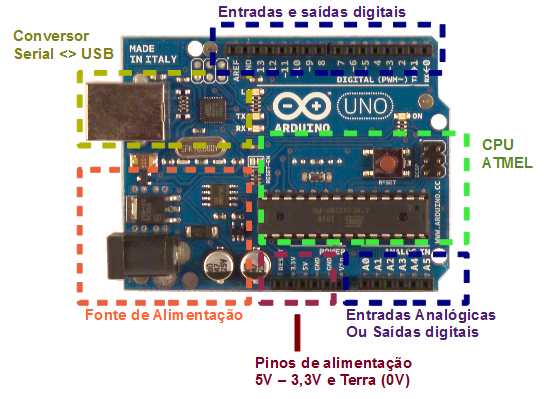
\includegraphics[scale = 0.75]{Figuras/Fig1_arduino.png}
    \legend{Fonte:  https://wiki.sj.ifsc.edu.br/index.php/MCO018703\_2018\_1\_AULA08}
    \label{fig:arduino}
\end{figure}

\textbf{Fonte de Alimentação}:Tem o principal papel de receber energia de alimentação externa, que pode variar entre as tensões entre 7 a 20 Volts com uma corrente elétrica mínima de 300mA. Existem adaptadores que ligam a fonte a uma pilha de 9V ou diretamente na tomada.

\textbf{Plugn USB e Conversor Serial/USB}: Tem como responsabilidade carregar o código da IDE do Arduíno para a placa. Pode ser utilizada como fonte de alimentação energética.

\textbf{Unidade Central de Processamento ATMEL}: É o circuito integrado responsável por executar o código enviado a placa. Cada placa tem  diferentes tipos de microcontroladores, memórias internas e capacidade de processamento. Normalmente são chips da marca ATMEGA

\textbf{Pinos de Alimentação}: Regulam tensões mínimas e máximas da voltagem provenientes de fontes externas ou da alimentação USB. As tensões possíveis dos pinos de alimentação são: 3,3V, 5V e 0V(GND).

textbf{Entradas e Saídas Digitias}: São portas lógicas usadas para enviar ou receber sinais digitais para sensores, ou dispositivos conectados a placa com a informação de 0V(desligado) a 5V(ligado).

\textbf{Entradas Analógicas}: São portas que tem o papel de realizar leituras de sinais analógicos de sensores ligados a placa como luz, movimento, temperatura, entre outros.

Inicialmente para o trabalho foi cogitado utilizar a placa NODEMCU, pois, o número de portas lógicas digitais e analógicas eram suficientes para o projeto com a facilidade da conexão de Internet sem fio do módulo ESP8266-12E seria útil na transmissão de dados. Entretanto, o sensor de biruta eletrônica que é analógico não produziu resultados satisfatórios de mensuração. O comportamento para a falha foi devido ao nível de tensão que a placa utiliza na porta analógica A0, a única do NODEMCU possui uma tensão de 1V. O sensor analógico de biruta eletrônica, segundo o fabricante, é adequado para tensões de 5V e internamente é equipado com resistores que variam de 10K$\Omega$ até 80K$\Omega$ com a função de reduzir a voltagem de entrada resultando em uma voltagem de saída mais baixa. Para um nível de tensão de entrada de 1V em resistências dessa grandeza o resultado não seria preciso, por que além da incompatibilidade existe a varição de voltagem do equipamento que é de aproximadamente $\pm$ 0.2V.

Por esse motivo no trabalho foi utilizado uma placa Arduino UNO pois ela suportou bem todos os sensores utilizados no trabalho.


\subsection{Internet das Coisas}

A iot já está mudando a maneira como pessoas e objetos se relacionam entre si\cite{zmud2018primer}. Imagine uma geladeira capaz de informar para o smartphone que a quantidade de ovos em seu interior está abaixo do suficiente para fazer um bolo. Então um aplicativo do smartphone com essa informação enviada pela geladeira já faz uma rota de possíveis locais que vendem ovos e manda uma notificação para o usuário cada vez que ele se aproxima de um local de compra. 

Não basta o objeto estar conectado à Internet que já é sinônimo de iot, mas além de processar dados ele pode tomar pequenas decisões de forma inteligente para que haja intervenção humana. Por exemplo, se a temperatura atingir 40°C, em uma sala técnica de informática, será enviado uma notificação para que o responsável possa tomar alguma ação. 

Uma boa síntese da variedade de questões foi feita por \cite{atzori2010internet}. A figura \ref{fig:IoTParadigma} é uma tentativa de resumir as principais áreas de pesquisa e tipos de aplicação e oferecer uma visão mais completa da IOT, que segundo o autor da imagem é melhor entendida como um paradigma computacional formado pela sobreposição de visões orientadas às coisas, à Internet e à semântica.
A visão de Atzori é muito voltada para a tecnologia, não vê as finalidades nos quais o usuário pode se deter como usabilidade, autorização e autenticação para o acesso à informação.
\\
\\
\\
\\
\\
\\
\\
\\
\begin{figure} [!h]
    \centering
    \caption{O paradigma da Internet das Coisas}
    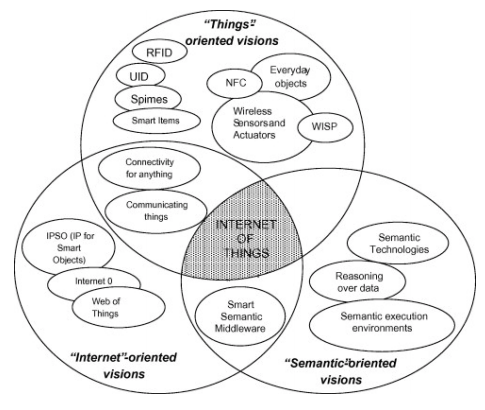
\includegraphics[scale = 0.7]{Figuras/Internet_das_Coisas.png}
    \legend{Fonte: (ATZORI, 2010, p. 2)}
    \label{fig:IoTParadigma}
\end{figure}


Outra abordagem mais simples do conceito de iot é dividi-lo em três camadas. Segundo \cite{zmud2018primer} a primeira representada por sensores com a responsabilidade de capturar dados. Que transmite esses dados para a segunda camada de comunicação responsável por filtrar, agregar informações e a última camada representada pela nuvem como a responsabilidade de manter, analisar e gerar ferramentas de visualização de conhecimento para definir ações futuras.

\begin{figure} [!h]
    \centering
    \caption{Internet das Coisas em 3 Camadas}
    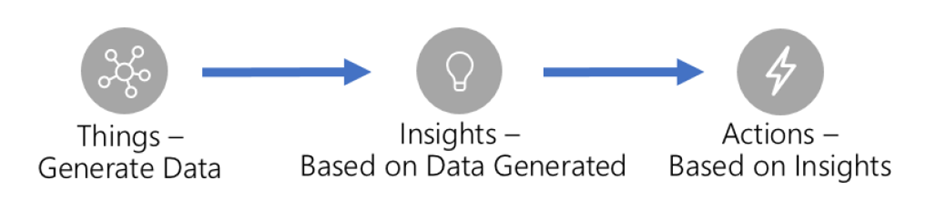
\includegraphics [scale = 0.40] {Figuras/framework_IOT.png}
    \legend{Fonte: Microsoft Azure IOT Framework}
    \label{fig:4}
\end{figure}

Um fator que permeia muitas pesquisas na área de Internet das coisas é a segurança, que é um elemento que deve envolver todas as camadas. Colaborando com estratégias para caso um componente for comprometido não faça prejuízo à estrutura. Para esse fim são utilizadas tecnologias como criptografia, controle de acesso com autorização e autenticação, identificação dos dispositivos entre outras medidas para garantir a integridade do sistema.

No que se refere às aplicações, podemos notar a presença de iot no nosso cotidiano. Como, por exemplo, sensores que detectam a presença física em uma determinada área e enviam informações para uma central de controle. Com isso é possível criar aplicação para controle de acesso de pessoas, dispositivos inteligentes podem se mover para a área que deve ser controlada por um determinado período no caso de aeroportos onde é necessário quando existe demanda\cite{hui2008rfid}.

Também já existem plataformas industriais para Internet das Coisas como é o caso de empresas como a Amazon com a AWS iot e Amazon Alexa, Microsoft como Azure IOT e IBM com a IBM Watson iot.


\subsection {Estrutura Meteorológicas Brasileira para o Contexto Aeronáutico}

Um fator que contribuiu para o início do desenvolvimento da meteorologia brasileira foi um naufrágio, na costa do Rio Grande do Sul motivado por um temporal em 11 de julho de 1887 \cite{barboza2006historia}. Na época o Brasil não tinha serviço de previsão do tempo. A tragédia motivou alguns cientistas a tentar explicar o que aconteceu, porém, como os dados da época eram escassos e o conhecimento da dinâmica atmosférica também não tiveram sucesso.

Vinte anos depois da ocorrência, cientistas brasileiros adquiriram conhecimento para elaboração de mapas sinóticos desde modo foi possível explicar o que aconteceu em 11 de julho de 1887 e também iniciar o serviço de previsão do tempo no Brasil\cite{oliveira2009inmet}.

\begin{figure} [!ht]
    \centering
    \caption{Exemplo de mapa sinótico}
    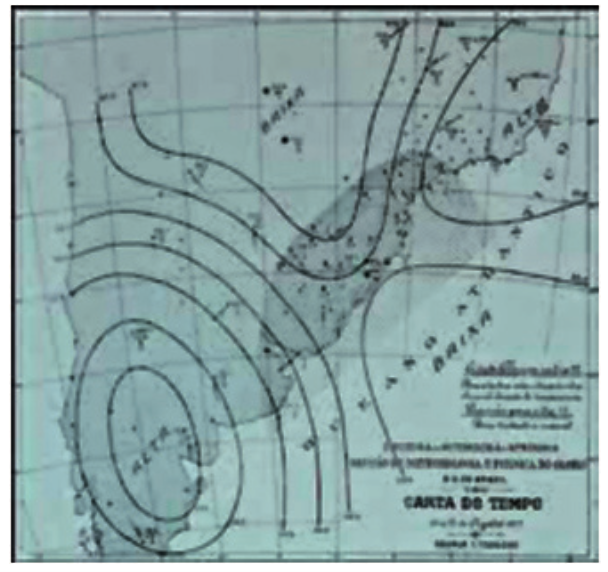
\includegraphics [scale = 0.35] {Figuras/mapa_sinotico.png}
    \legend {Fonte: (Oliveira,2009 p.36)}
    \label{fig:4}
\end{figure}

A meteorologia no Brasil foi se aprimorando com técnicas vindas do exterior e qualificação de profissionais e se chegou até a seguinte estrutura:

\begin{itemize}
    \item Instituto Nacional de Meteorologia (INMET) do Ministério da Agricultura
    \item Centro de Previsão do Tempo e Estudos Climáticos do Ministério da Ciência e Tecnologia(CPTEC)
    \item Meteorologia Aeronáutica do Comando da Aeronáutica e Meteorologia Marítima do Comando da Marinha, ambas pertencentes ao Ministério da Defesa e às Meteorologias Estaduais: FUNCEME(Ceará), SIMEPAR(Paraná), EPAGRI/CIRAM(Santa Catarina) entre outros.
\end{itemize}

O órgão oficial de meteorologia brasileiro é o INMET \cite{oliveira2009inmet}. É o representante do país junto à organização Meteorológica Mundial(OMM), criada em 1950 é o organismo responsável das Nações Unidas pela meteorologia, no que diz respeito ao clima, tempo e ciências afins.

No contexto aeronáutico, o serviço de meteorologia é regulamenta pela Organização da Aviação Civil Mundial(OACI), sendo o DECEA, o órgão normatizador e fiscalizador, conforme os padrões de OMM, OACI e os interesses nacionais. O serviço tem como finalidade a observação da atmosfera, visando eficiência e a segurança das atividades aéreas.

A segurança das atividades aéreas usando informações meteorológicas, a grosso modo, é basicamente informar ao piloto as condições do tempo que possam ser encontradas desde do momento da decolagem até o momento do pouso. Condições que são observadas, em parte, e prognosticadas no todo destacando as adversidades para o voo como: áreas de turbulências, aéreas de formações de gelo, trecho de visibilidade reduzida, teto baixo. 

Segundo \cite{costa2008meteorologia} o planejamento do voo começa com a observação e análise das condições do tempo. Condições que são observadas somente nas proximidades dos aeródromos, num raio de 20 km enquanto a previsão cobre toda a rota utilizada por um voo.

Para que a informação cumpra seu papel existe diferentes setores na meteorologia aeronáutica conforme exposto por \cite{henrique2005meteorologia}:
\begin{itemize}
    \item Rede de Estações Meteorológicas(REM).
    \item Estação de Radares Meteorológicos(ERM).
    \item Bancos de Dados Meteorológicos.
    \item Sistema de divulgação de informes meteorológicos
\end{itemize}
    
A rede de estações meteorológicas é formada por estações de superfície e de altitude(EMA). E divulgação de informações operacionais é feita por meio oficial através da REDEMET \cite{redemet2020homepage} que é uma plataforma mantida pela FAB que tem como objetivo a integração dos serviços de meteorológica com o acesso a informações de modo rápido e eficiente.


\subsection{Estação Meteorológica de Superfícies}

Segundo a instrução do comando da aeronáutica(ICA) \cite{BRASILMCA104}, as estações meteorológicas têm a responsabilidade de coletar, processar e registrar dados meteorológicos de superfície e altitude para apoio à navegação aérea. Podendo ser de três tipos:
\begin{itemize}
    \item Estações Meteorológicas de Altitude (EMA)
    \begin{citacao}
As Estações Meteorológicas de Altitude têm por finalidade coletar, através de Radiossondagem, dados de pressão, temperatura, umidade, direção e velocidade do vento, nos diversos níveis da atmosfera. 
    \end{citacao}
    \item Estações Meteorológicas de Superfície (EMS)
    \begin{citacao}
As Estações Meteorológicas de Superfície têm por finalidade efetuar a coleta e o processamento de dados meteorológicos à superfície para fins aeronáuticos e sinóticos. Devem ser instaladas nos aeródromos e fazem parte da rede básica da Organização Meteorológica Mundial (OMM), quando equipadas apropriadamente.
\end{citacao}

\end{itemize}

Conforme exposto somente as EMS são instaladas nos aeródromos e elas são classificadas em três categorias conforme \cite{BRASILMCA104} EMS-1, EMS-2, EMS-3. A principal diferença entre está nos dispositivos que compõem cada categoria da estação. Para expor de modo claro a diferença de cada categoria de estação por sensores é interessante explicar o papel de cada sensor conforme \cite{DECEA}

\begin{itemize}
    \item Anemômetro: fornece a direção e velocidade (média e máxima) do vento nas zonas de ponto de toque das pistas; 
    \item Transmissômetro: fornece os valores de Alcance Visual na Pista ao longo das pistas;
    \item Tetômetro: fornece a altura da base das nuvens, referente ao sítio do marcador médio. Na impossibilidade de instalação no marcador médio, o tetômetro poderá ser instalado junto ao sítio meteorológico da cabeceira principal ou próximo ao sítio do marcador interno; 
    \item sensores de temperatura do ar e de umidade relativa: fornecem a temperatura do ar e a umidade relativa, referentes ao sítio meteorológico principal;
    \item barômetro: fornece a pressão atmosférica, informando valores de Pressão reduzida ao nível do mar pelo gradiente vertical da atmosfera padrão(QNH),Pressão real ao nível do mar(QFF) e a Pressão atmosférica ao nível de elevação do aeródromo ou na cabeceira da pista)(QFE), localizado no sítio meteorológico principal; 
    \item pluviômetro: fornece a quantidade de precipitação, referente ao sítio meteorológico principal;
\end{itemize}

A EMS-1 e a categoria de estação mais completa ela possui todos os sensores listado acima. A EMS-2 possui todos os sensores listados acima exceto o transmissômetro. Já a EMS-3 a categoria mais simples possui os sensores.
\begin{itemize}
    \item Anemômetro: para informar o vento do aeródromo não necessariamente o das zonas de ponto de toque da pista.
    \item Os sensores de temperatura e de umidade relativa do ar e barômetro: também referente ao aeródromo não ao local meteorológico principal.
\end{itemize}

Além dos tipos de equipamento o \cite{DECEA} define como deve ser feita as observações meteorológicas podendo ser feitas de forma regular, especial ou local.

A observação regular é realizada em horários pré-fixados, em intervalos de uma hora e deve ser confeccionada e divulgada no formato de METAR que são mensagens meteorológicas para uso Operacional.

A observação especial quando ocorre variações meteorológicas consideráveis como, por exemplo: quando a velocidade média do vento à superfície mudar em 10 kt ou mais, em relação à última observação. Quando existir fenômeno ou combinação deles como nevoeiro, tempestade de poeira, precipitação congelante, trovoadas, nuvens do tipo funil entre outros. A observação especial deve ser divulgada em formato SPECI conforme documentações.

A observação local é aquela realizada quando ocorrer um acidente ou incidente aeronáutico no aeródromo, ou em sua vizinhança. Posteriormente, poderá ser fonte de informações para eventual investigação. Ela tem início no momento que o acidente ou incidente ocorre. 

Este trabalho utilizará das observações regulares no formato METAR para testar se os dados coletados pelo protótipo elaborado no trabalho podem ser consideradas iguais aos da plataforma REDEMET.




\subsection{Sensores}

Na eletrônica um sensor é um dispositivo com qualquer componente elétrico ou circuito eletrônico que permite a análise de uma determinada condição do ambiente\cite{neto2020eletronica}. Podendo ser
divididos em dois tipos: analógicos e digitais. Essa divisão é feita pelo modo como o dispositivo responde à variação de uma determinada condição.

Os sensores analógicos têm como base o sinal analógico. São sinais que, mesmo com a limitação entre dois valores de tensão, eles podem assumir infinitas representações intermediárias. Para cada nível da condição medida haverá um sinal de tensão correspondente. Como exemplo posso destacar, um sensor de luminosidade, que é um dispositivo cuja resistência varia de acordo com a quantidade de luz, quanto mais intensa à iluminação verifica-se que a resistência reduz de forma gradual.

\begin{figure} [h!]
    \centering
    \caption{Exemplo de sensor analógico}
    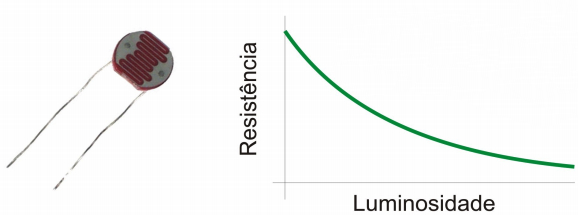
\includegraphics [scale = 0.5] {Figuras/sensor_analogico.jpg}
    \legend{Fonte: Adaptada.   encurtador.com.br/fI127}
    \label{fig:cinco}
\end{figure}


Os sensores digitais têm como base, níveis de tensão bem definidos. Eles podem ser descritos como Alto ou Baixo, Verdadeiro ou Falso, "1" ou "0". Eles usam da lógica binária, que é o alicerce do funcionamento dos sistemas digitais. Esse tipo de sensor alterna entre estados bem definidos. Como exemplo podemos descrever um sensor de infravermelho Conforme figura \ref{fig:infraVermelho}. Se o feixe de infravermelho atinge o receptor, teremos um nível de tensão baixo. Quando algo bloqueia o caminho da luz infravermelha pode se considerar nível de tensão alto.

\begin{figure} [h!]
    \centering
    \caption{Exemplo de senor digital}
    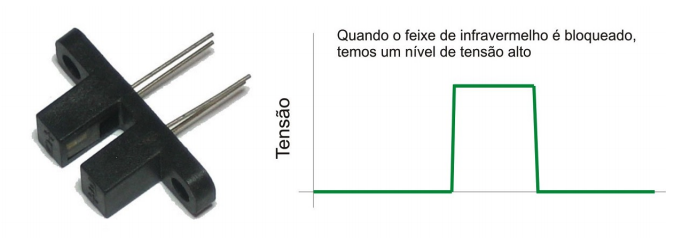
\includegraphics [scale = 0.5] {Figuras/sensor_digital.png}
    \legend{Fonte:  https://bityli.com/OGb1E }
    \label{fig:infraVermelho}
\end{figure}

O fato é que em projetos que envolve sensores sempre iremos encontrar os dois tipos. Na plataforma arduino utilizamos as portas lógicas digitais isso fornece a capacidade de receber e enviar sinais digitais e quando se utiliza portas analógicas é possível capturar sinais analógicos e mapeá-los para sinais digitais.

Nesse trabalho o critério de seleção dos sensores para a compor o protótipo da estação foi: 
 \begin{enumerate}
   \item Disponibilidade do sensor no mercado brasileiro.
   \item Menor Preço.
   \item Sensores que podem medir mais de uma varíavel.
   \item Estudos comprovando a eficiência do sensor.
 \end{enumerate}

\subsubsection {Anemômetro}

O anemômetro utilizado no trabalho e do tipo concha que é composto por três ou mais conchas de formato especial montada simetricamente formando ângulos de 90 graus com um eixo vertical. A velocidade do vento, independentemente de direção, faz mover o conjunto das conchas um mecanismo que conta as rotações e então a velocidade é calculada com o auxílio de um dispositivo de contagem no caso do modelo escolhido para esse trabalho utiliza um sensor Reed Switch \cite{USINAINFOBLOG}.

\begin{figure} [!h]
    \centering
    \caption{Anemômetro tipo concha - Modelo SV10}
    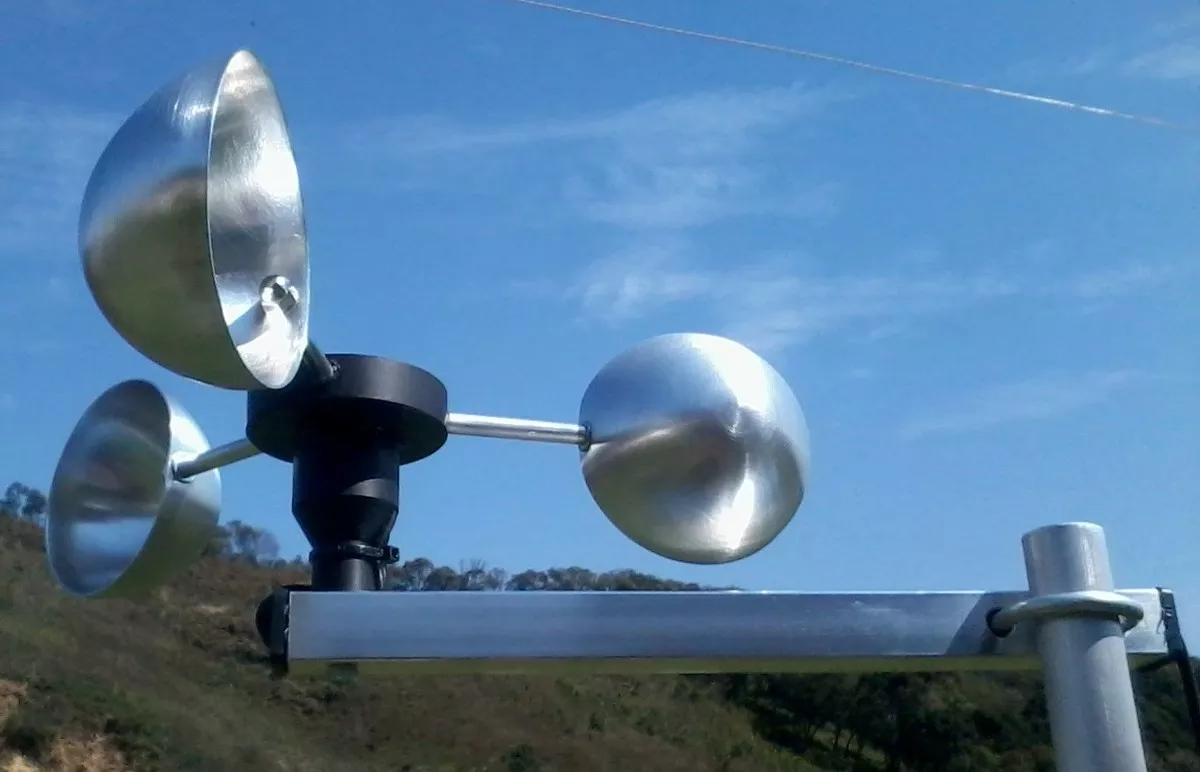
\includegraphics[scale=0.25]{Figuras/ane_SV10.png}
    \legend{Fonte: Adaptada https://www.usinainfo.com.br/blog/ }
    \label{fig:anemometro}
\end{figure}

O modelo de anemômetro SV10 foi escolhido para o trabalho por que foi o único encontrado no mercado. Segundo o manual do fabricante \ref{manAnemot} ele trabalha com várias tensões 3V3, 5V e 12V, e formado por três conchas feitas de alumínio, segundo a descrição do equipamento ele pode medir ventos de até 120 Km/h\cite{USINAINFOBLOG}.



\subsubsection{Biruta}

Birutas eletrônicas que usam a energia elétrica para medir a direção do vento. O modelo escolhido para o trabalho DV10 por que foi o único encontrado no mercado. Ele Consegue medir a direção do vento nos pontos cardeais e colaterais, ou seja, nos graus (0º, 45º, 90º, 135º, 180º, 225º, 270º e 315º). Esse equipamento recebe uma voltagem de entrada de 5V e conforme a direção do vento a aplicado o conceito de divisão de tensão com resistores variando de 10K$\Omega$ até 80k$\Omega$ gerando uma voltagem final conforme anexo \ref{manAnemog} correspondente a direção do vento.

\begin{figure} [!h]
    \centering
    \caption{Biruta Modelo DV10}
    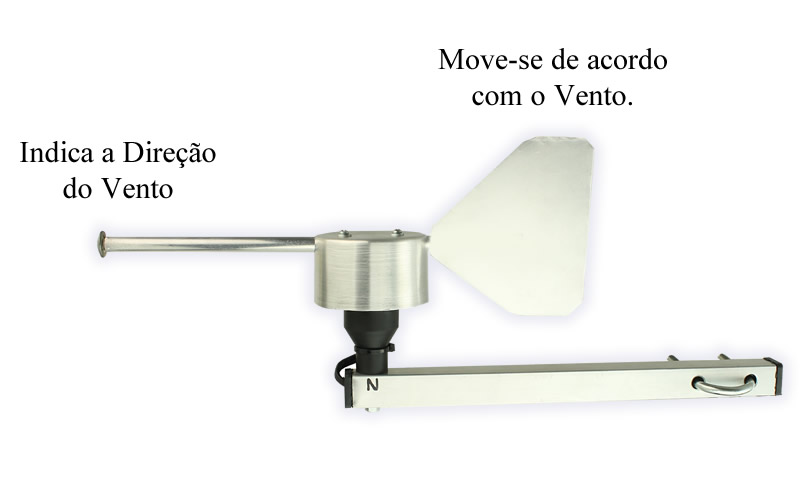
\includegraphics[scale=0.25]{Figuras/posicao-da-pa-e-indicacao.jpg}
    \legend{Fonte: Adaptada https://www.usinainfo.com.br/ }
    \label{fig:biruta}
\end{figure}


\subsubsection{Sensor de Temperatura}

Para sensor de temperatura foram encontrados vários modelos no mercado. Para decidir qual sensor deverá fazer parte da estação foi utilizado o trabalho de \cite{konstantinoscomparative} que compara três sensores para medir temperatura do mercado são MCP9808, BMP180 e o DHT22 com as medições feitas em um termômetro de mercúrio.

O sensor que teve uma maior aproximação com as medições feitas no termômetro de mércurio foi o BMP180 com uma taxa de erro medida através do uso de regressão linear. No mercado o sucessor do BMP180 é o sensor BMP280 que tem a mesma finalidade, porém, com um consumo energético mais eficiente e precisões melhores e tamanho reduzido. Na tabela 2.1 podemos notar as principais diferenças entre os modelos.

\begin{table}[!h]
\centering
\begin{tabular}{|l|c|c|}
\hline
\textbf{Parâmetro}                           & \textbf{BMP180} & \textbf{BMP280} \\ \hline
Dimensões                                    & 3,6 mm x 3,8mm  & 2,0 mm x 2,5 mm \\ \hline
Tensão Mínima                                & 1,6V            & 1,2V            \\ \hline
Consumo de Corrente Elétrica Médio           & 12$\mu$A         & 2,7$\mu$A        \\ \hline
Precisão para medição de pressão atmosférica & 1Pa             & 0.016Pa         \\ \hline
Precisão para medição de temperatura         & 0,1 ºC          & 0,01 ºC         \\ \hline
\end{tabular}
\caption{Diferenças entre os sensores BMP180 e BMP280}
\label{tab:tablebmp}
\end{table}

O sensor de temperatura escolhido para formar a estação do trabalho será o BMP280 conforme visto na tabela \ref{tab:tablebmp} ele tem alta precisão e baixo consumo energético.

\subsubsection{Sensor de Pressão Atmosférica}

O sensor BMP280 além de medir temperatura ele também mede pressão atmosférica com a finalidade de reduzir custos também foi escolhido para a mensuração dessa variável conforme visto na tabela\ref{tab:tablebmp} ele pode mensurar uma faixa entre 940 e 1100 hPa. Tem uma precisão de $\pm$0,016Pa.

\begin{figure} [!h]
    \centering
    \caption{Sensor BMP280}
    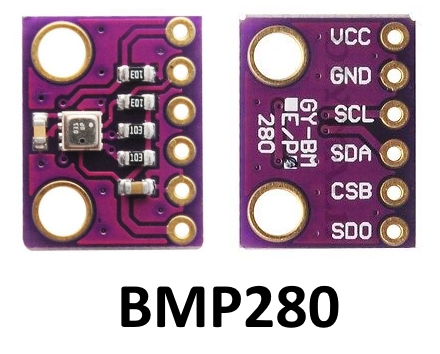
\includegraphics[scale=0.5]{Figuras/BMP280_Pinout.jpg}
    \legend{Fonte: https://forum.arduino.cc/index.php?topic=654763.0}
    \label{fig:bmp280}
\end{figure}

\subsubsection{Sensor de Umidade Relativa do Ar}

Na plataforma arduino os sensores de umidade relativa do ar mais encontrado no mercado são o DHT11 e DHT22. Os dois modelos são da mesma fabricante. A diferença entre ambos conforme \cite{AutoCoreBlog} pode ser entendida na figura abaixo:

\begin{table}[!h]
\centering
\begin{tabular}{|l|c|c|}
\hline
\textbf{Parâmetro}           & \textbf{DHT 11} & \textbf{DHT 22} \\ \hline
Tensão de Alimentação        & 3V - 5.5V       & 3.3V - 6V       \\ \hline
Corrente Máxima              & 2.5mA           & 1.5mA           \\ \hline
Faixa de Leitura Umidade     & 20 - 80\%       & 0 - 100\%       \\ \hline
Precisão Umidade             & 5\%             & 2\%             \\ \hline
Faixa de Leitura Temperatura & 0 até 50 ºC     & -40 até 125 ºC  \\ \hline
Precisão Temperatura         & 2 ºC            & 0,5 ºC          \\ \hline
Intervalo de Medições        & 1s              & 2s              \\ \hline
\end{tabular}
\caption{Diferenças entre DH11 e DHT22}
\label{tab:dhtsensor}
\end{table}

Fica bem exposto na tabela \ref{tab:dhtsensor}, que o DHT11 ele é duas vezes mais rápido que o DHT22 em suas medições. Sua precisão em relação a umidade relativa do ar não é boa podendo chegar a $\pm$ 5\% além de consumir mais energia comparado ao DHT22. No trabalho de \cite{ribeiro2016avaliaccao} e demonstrado que realmente a faixa de erro de 2\% se comprova. Vale notar que os dois podem ser alimentados com a faixa de tensão entre 3.3V a 5.5V. Em relação a custo também o DHT11 é bem mais barato que o DHT22. O DHT11 custa em média 70\% que DHT22.



\subsection{Plataforma ThingSpeak}

ThingSpeak é uma plataforma para Internet das coisas que permite a agregação, a visualização de dados em tempo real na nuvem. Possibilitando o envio e leitura de dados por dispositivos, criando visualizações gráficas em tempo real. A plataforma permite o envio de alerta quando determinadas condições são atingidas para redes sociais como Twitter e Twilio. Além disso, dentro do ambiente da plataforma é possível a execução de código da linguagem MATLAB que é usada para pre-processamento, visualização e analise \cite{ThinkSpeak}. A grande vantagem de se usar o Thingspeak e a facilidade para configuração de um servidor sem a necessidade de desenvolvimento de um sistema completo para WEB.

A plataforma Thingspeak também permite o armazenamento dos dados coletados e a disponibilização dos dados em formato de XML ou JSON e também permite a leitura dos dados através de uma requisição HTTP. Os dados coletados são armazenados em canais que permitem o armazenamento de até oito tipos de dados diferentes. Além de informações de descrição, altitude, latitude e longitude. Assim que um canal é criado ele tem uma sequência de números únicos um ID. Os dados podem ser acessados através da API do Thingspeak que necessita de uma chave de acesso gerada pela própria plataforma para as operações de leitura e operações de escrita de dados. Os canais eles pode ter visualizações públicas ou privadas. Quando o canal é público não é necessário utilizar chave de leitura para o acesso.

\begin{figure}[h!]
    \centering
    \caption{Plataforma Thingspeak}
    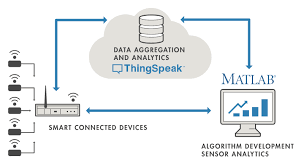
\includegraphics{Figuras/think_speak.png}
    \legend{Fonte: https://thingspeak.com/ }
    \label{fig:thinkSpeak}
\end{figure}

O Thingspeak tem suporte a linguagens de programação como Ruby, Python e Node.js. Linguagens bem populares no meio WEB e a facilidade de integração com Python permite o acesso a várias bibliotecas que o Python possui para trabalhar com análise de dados não obrigando o desenvolvedor a utilizar a linguagem que já vem com a plataforma o MATLAB.

A plataforma possui alguns tipos de licenciamento esse trabalho utilizou a licença free que possui as limitações de enviar até 3 milhões de mensagens por ano ao serviço ThingSpeak, a criação de até quatro canais e as operações de atualização deve ter um intervalo mínimo de 15 segundos. Cada mensagem deve conter até 3000 bytes essa limitação vale para todos os tipos de licença. Existe também limitação em relação ao armazenamento na conta gratuita é possível armazenar até 10 milhões de mensagens por até três anos se não ocorrer nem uma atualização dos dados no canal. Esse trabalho utilizou um total de 13 516 mensagens menos de 1\% da capacidade oferecida pela plataforma.

Existem outras plataformas de IOT concorrentes do Thingspeak destaco a plataforma Blynk que foi considerada para uso no projeto. Ela possui com três componentes um aplicativo, um servidor e um conjunto de placas. Tem a vantagem de ter configurações como a conexão com a Internet para placas mais utilizadas no mercado como arduino UNO, NODEMCU, ESP8266. Permitindo também essa comunicação por portas seriais com uma estação de trabalho \cite{8473224}. O Blynk é parte gratuito para uso de bibliotecas, servidor e hospedagem na nuvem. A forma de monetizar está no aplicativo esse serviço tem uma série de widgets para visualização de informações ou botões para acionar comandos. Cada widget consome uma moeda virtual ao iniciar uma conta o usuário recebe um valor inicial.

\begin{figure}[h!]
    \centering
    \caption{Widgets da Plataforma Blynk}
    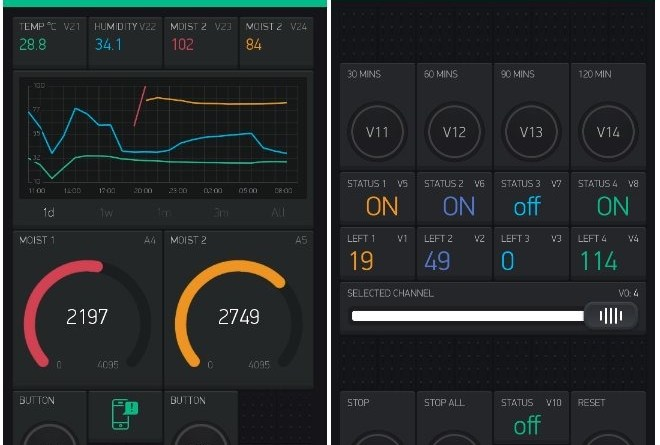
\includegraphics[scale=0.5]{Figuras/blynk_app.jpg}
    \legend{Fonte: https://blynk.io/ }
    \label{fig:blynk}
\end{figure}


\subsection{Protocolo MQTT}

O MQTT segundo \cite{torres2016analise} é um protocolo próprio para comunicação entre máquinas(M2M) opera com o TCP/IP e funciona bem com redes de alta latência, com instabilidade na comunicação e baixa largura de banda.

Conforme descrito em \cite{de2017internet} O MQTT funciona através de três estruturas:

\begin{itemize}
\item MQTT Broker: É o servidor onde os dados ficam disponíveis para eventuais dispositivos assinantes no caso desse projeto será a plataforma ThingSpeak.
\item Publisher MQTT: É o dispositivo que gera a informação e publica no servidor. No caso desse trabalho dividimos a responsabilidade de publicar em um script em Python e gera os dados que será feito através do código embarcado no arduino.
\item Subscriber MQTT: São os dispositivos interessados nos dados do serviço no caso em análise será o aplicativo disponibilizado para visualização na plataforma Thinspeak.
\end{itemize}

As vantagens de utilização do protocolo é na baixa necessidade de processamento para o envio de mensagens e no baixo consumo de banda com seu cabeçalho muito pequeno cerca de 2 bytes segundo \cite{mota2017analise}. A desvantagem é que o protocolo não possui uma camada de segurança então utiliza os mecanismos do TCP/IP.



\section{Trabalhos Relacionados}

Nessa seção apresento projetos que já desenvolveram estações meteorológicas utilizando a plataforma arduino. Foram escolhidos trabalhos dos últimos cinco anos que utilizaram conceitos similares para o desenvolvimento de um protótipo. Primeiramente será feito um comentário sobre cada trabalho e por fim será apresentada uma tabela \ref{tab:comp_trabalhos} com as principais características dos trabalhos.

No trabalho de \cite{torres2015aquisiccao} o autor propõe a criação de uma estação meteorológica simplificada com a utilização da plataforma arduino com objetivo de reduzir custos das estações meteorológicas disponíveis no mercado. O trabalho conta com a utilização de três sensores: temperatura, luminosidade e umidade do ar. São realizados testes em laboratório para comparar dados de uma estação, do Instituto Nacional de Meteorologia(INMET), mais próxima geograficamente do local do trabalho. Os resultados são apresentados graficamente baseados na interpretação do autor, não há a presença do conceito de iot que poderia facilitar a disponibilização da informação e redução de custos. Nesse projeto todos os dados coletados foram mantidos em um módulo de cartão de memória.

Na elaboração de estação meteorológica feita por \cite{da2016estaccao} podemos encontrar a utilização de sensores para: temperatura, precipitação atmosférica, intensidade da luz solar, umidade do ar, pressão atmosférica, velocidade do vento. O autor também adquiriu um módulo à parte para conexão com a Internet, o modulo ESP8266, e criou um sistema WEB próprio para receber os dados dos sensores. O autor comparou os custos dos sensores da plataforma Arduino com os sensores de uma estação meteorológica convencional. No trabalho em questão não é detalhado a amostra utilizada para se chegar a taxa de erro na comparação nem detalha onde os testes foram feitos apenas mencionam que foram usados dados do INMET. Ocorreu a mesma situação na comparação de custos e escolha dos sensores.

No trabalho \cite{deestaccao} o autor propõe a criação de uma estação meteorológica de baixo custo voltada para o contexto da agricultura com a utilização da plataforma Thingspeak para a visualização e armazenamento dos dados. O autor também faz uma análise de custo simplificada. Nesse trabalho é utilizada a placa arduino modelo WeMos que já vem com um módulo WiFi embutido. No projeto foram utilizados sensores de temperatura, pressão, umidade relativa e um módulo para medir a radiação UV. Existe um detalhamento da amostra de dados utilizada para a comparação com uma estação meteorológica convencional, porém não são apresentados dados sobre a condição de vento que como o autor mesmo informa tais dados fazem parte de uma estação meteorológica convencional desse modo temos que o trabalho desenvolve uma estação não completa em termos de capacidade. Por isso não é adequado comparar custos de instrumentos que não tem a mesma capacidade.  

\begin{table}[!h]
\centering
\begin{tabular}{|l|c|c|c|}
\hline
                      & \textbf{(TORRES et al., 2015)} & \multicolumn{1}{l|}{\textbf{(SILVA et al., 2016a)}} & \multicolumn{1}{l|}{\textbf{(NETO et al., 2018)}} \\ \hline
Sensor de Temperatura & Possui                         & Possui                                              & Possui                                            \\ \hline
Sensor de Pressão     & Não Possui                     & Possui                                              & Possui                                            \\ \hline
Sensor de Umidade     & Possui                         & Possui                                              & Possui                                            \\ \hline
Biruta                & Não Possui                     & Não Possui                                          & Não Possui                                        \\ \hline
Anemômetro            & Não Possui                     & Possui                                              & Não Possui                                        \\ \hline
iot                   & Não Possui                     & Possui                                              & Possui                                            \\ \hline
Comparação de Custos  & Possui                         & Possui                                              & Possui                                            \\ \hline
Comparação de Dados   & Possui                         & Não Possui                                          & Não Possui                                        \\ \hline
\end{tabular}
\caption{Trabalhos Relacionados}
\label{tab:comp_trabalhos}
\end{table}


No trabalho proposto teremos todas as características listadas na tabela \ref{tab:comp_trabalhos}. Será considerado quais são as informações mínimas que uma EMS-3 deve possuir com base nas publicações do Departamento de Controle do Espaço Aéreo(DECEA). Aplicado o conceito de Internet das coisas com o uso da plataforma Thingspeak para facilitar a distribuição e o armazenamento dos dados mensurados pelos sensores e realizado teste de hipótese estatística para a comparação entre as amostras. Como a plataforma REDEMET é mais utilizada no contexto aeronáutico sera considerada para a comparação de dados com o protótipo.







.


\chapter{Desenvolvimento} \label{desenvolvimento}

O desenvolvimento do protótipo foi dividido em duas partes. A primeira parte chamada de Hardware que é a montagem do equipamento, formado basicamente por uma placa arduino UNO, sensores e fios de interconexão. No trabalho não foi aplicada nenhuma técnica de soldagem nos equipamentos. A Segunda parte chamada de Software e composta por um código em C ,embarcado no arduino UNO, e um script em Python. A função principal do código em C é capturar os dados dos sensores e ficar esperando caracteres enviados pelo script de Python. Cada caractere corresponde a um dos sensores conectados ao protótipo. O código do script fica armazenado numa estação de trabalho, também tem a responsabilidade de enviar via protocolo MQTT informações para a plataforma ThingSpeak. Essa separação do código em duas partes é útil para a placa arduino que possui memória bem limitada não ficar sobrecarregada. Um código muito extenso pode nem ser embarcado.


Nesse capítulo também e descrito a experiência realizada que tem por objetivo validar a eficiência do protótipo. O experimento compara os dados obtidos na plataforma REDEMET com os coletados pelo protótipo. 

\section{Hardware}

O Hardware da estação meteorológica é composto por sensores: BMP280, DHT22, SV10 e DV10, fios para conexão, dois resistores de 10k$\Omega$, um de resistor de 4.7k$\Omega$, uma protoboard de 480 pontos e um arduino UNO. O diagrama do hardware pode ser visto na figura \ref{fig:hardestacao}.

\begin{figure} [!ht]
    \centering
    \caption{Projeto do Hardware Estação Meteorológica}
    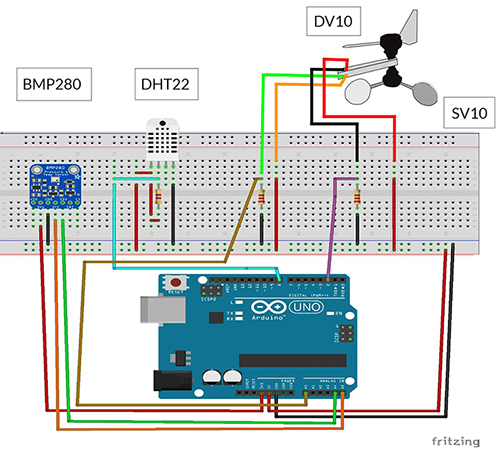
\includegraphics [scale=0.45]{Figuras/estacao_proj_hard.jpg}
    \legend{Elaborado no software Fritzing }
    \label{fig:hardestacao}
\end{figure}

Todos os sensores foram ligados conforme orientação do fabricante. Podemos destacar o sensor BMP280 pela possibilidade de escolher entre: o protocolo de enlace I2C ou SPI. O trabalho optou por utilizar o protocolo I2C por duas razões trabalha em velocidades maiores e a econômia com fios \cite{cinel2017desenvolvimento}. 

Outro detalhe que merece a atenção é o posicionamento da biruta eletrônica e anemômetro. Com o auxílio de uma bússola eles foram colocados de modo que o grau 0º da biruta eletrônica represente o ponto cardeal norte. Esses dois sensores foram colocados em uma altura de 4,56 metros em relação ao chão.

\begin{figure} [!h]
    \centering
    \caption{Hardware Montado}
    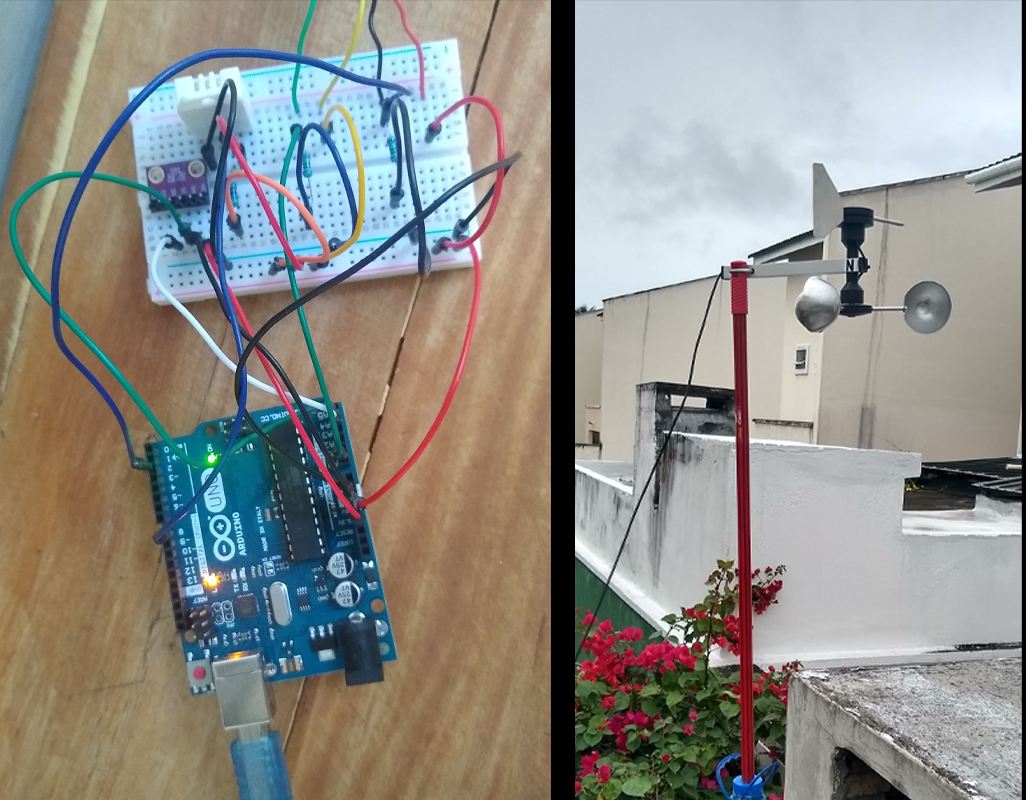
\includegraphics [scale=0.40]{Figuras/Hardware_Estacao.jpg}
    \legend{Fonte: Autoria própria }
    \label{fig:estacao_hardware}
\end{figure}

\section{Software}

Essa parte do desenvolvimento é composta por dois códigos principais um em Python no apêndice \ref{PythonScript} e outro escrito em C no apêndice \ref{CodigoArd}. A divisão além de ajudar no desempenho, melhora a legibilidade do código, isso contribuiu para que a placa arduino utilizasse apenas 32\% da memória interna para armazenamento isso segundo a ferramenta de desenvolvimento arduino IDE.

\subsection{Script em Python}

A primeira ação do código após a importação das bibliotecas necessárias é iniciar as configurações de comunicação serial na mesma porta de operação do arduino com a mesma taxa de transmissão.

No script que está no apêndice \ref{PythonScript} foram deixados explícitos os três modos de conexão da biblioteca do Python para MQTT são eles: usando apenas o protocolo TCP, WebSockets, ou SSL/TLS e WebSockets. A única forma segura de enviar dados é através de SSL/TLS e WebSockets para funcionar é necessário fazer uma configuração na plataforma ThingSpeak e na estação de trabalho que consiste em definir o tipo de certificado e seu caminho na máquina.

Para que a comunicação aconteça com a plataforma é necessário a definição de algumas variáveis como a chave da API de escrita, o endereço MQTT do servidor, e o ID do canal.

Após todas essas configurações as publicações são feitas dentro de um loop infinito onde o tempo de transmissão pode ser configurado. Inicialmente para testes foi estabelecido um valor de 30 segundos. Dentro do loop temos a chamada para uma função \emph{realizar\_mensuração(comando):} que transmite ao arduino um carácter correspondente a um sensor. Assim que todas os dados são obtidos é montado um payload para a publicação MQTT e enviado a plataforma ThingSpeak.

\subsection{Código embarcado no arduino}

No código do arduino é preciso realizar alguns procedimentos iniciais para a correta inicialização dos sensores. Procedimentos que utilizam bibliotecas de fabricantes para os sensores DHT22 e BMP280. Os sensores DV10 e SV10 apenas necessitam de definições de algumas constantes sem nenhuma chamada de método de biblioteca para configuração.

Para obter as leituras dos sensores DHT22 e BMP280 basta uma chamada de método. O sensor DV10 necessitou de alguns ajustes no método de medição devido à existência de uma variação de 0.15V na saída o que pode gerar imprecisão quando a direção do vento está nas direções de 270 graus e 315 graus. Para realizar o ajuste feito foi realizada 10 leituras do sensor e apenas considerando o valor mediano das medições. O sensor SV10 necessita de 5 segundos para retorna uma leitura isso por que é preciso contar quantas vezes o dispositivo reed switch foi acionado para calcular corretamente o número de rotações por minuto e inferir o daí o valor da velocidade do vento.

Todo o código do arduino pode ser encontrado no apêndice \ref{CodigoArd}. Na figura \ref{fig:acoes_software} pode ser visualizada as principais ações do software no protótipo.

\begin{figure} [!h]
    \centering
    \caption{Principais Ações de Software}
    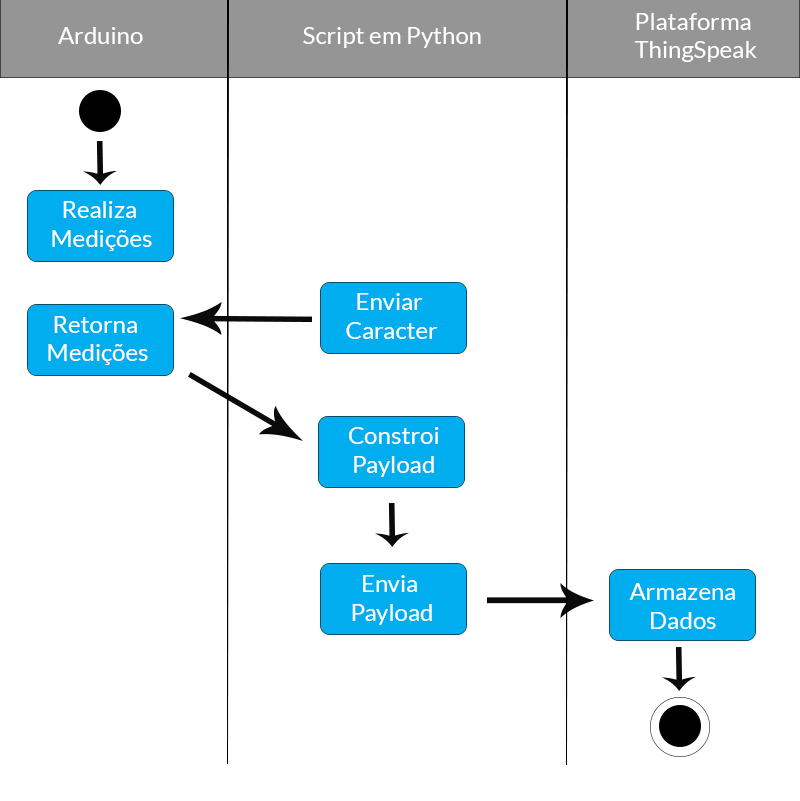
\includegraphics [scale=0.40]{Figuras/fluxo.jpg}
    \legend{Fonte: Autoria própria }
    \label{fig:acoes_software}
\end{figure}

\section{O experimento}

O experimento tem por objetivo produzir resultados para que seja feita uma comparação com a plataforma REDEMET. Ele consiste em deixa o protótipo coletando dados durante três dias e enviando a plataforma ThingSpeak de modo constante e depois será realizado um teste de hipótese para verificar a igualdade das médias das amostras das variáveis.

As variáveis do experimento serão quantitativas contínuas, são elas: temperatura, pressão, umidade relativa do ar, direção do vento e velocidade do vento. Todas os valores coletados serão arrendondados. Na tabela \ref{tab:unidades_medidas} contém informações sobre unidade de medida das variáveis.

\begin{table}[!ht]
\centering
\begin{tabular}{|l|c|}
\hline
\textbf{Variavel}      & \textbf{Unidade de medida} \\ \hline
Temperatura            & Celsius (ºC)               \\ \hline
Pressão                & Hectopascal(hPa)           \\ \hline
Umidade Relativa do Ar & Percentual (\%)            \\ \hline
Direção do Vento       & Graus(º)                   \\ \hline
Velocidade do Vento    & Nó (kt)                    \\ \hline
\end{tabular}
\caption{Fonte: Autoria própria}
\label{tab:unidades_medidas}
\end{table}

O protótipo ira enviar informações das variáveis para a plataforma ThingSpeak a cada 30 segundos. As informações enviadas  podem ser acompanhadas pelo aplicativo disponibilizado pela plataforma. 

\begin{figure} [!h]
    \centering
    \caption{Aplicativo ThingSpeak}
    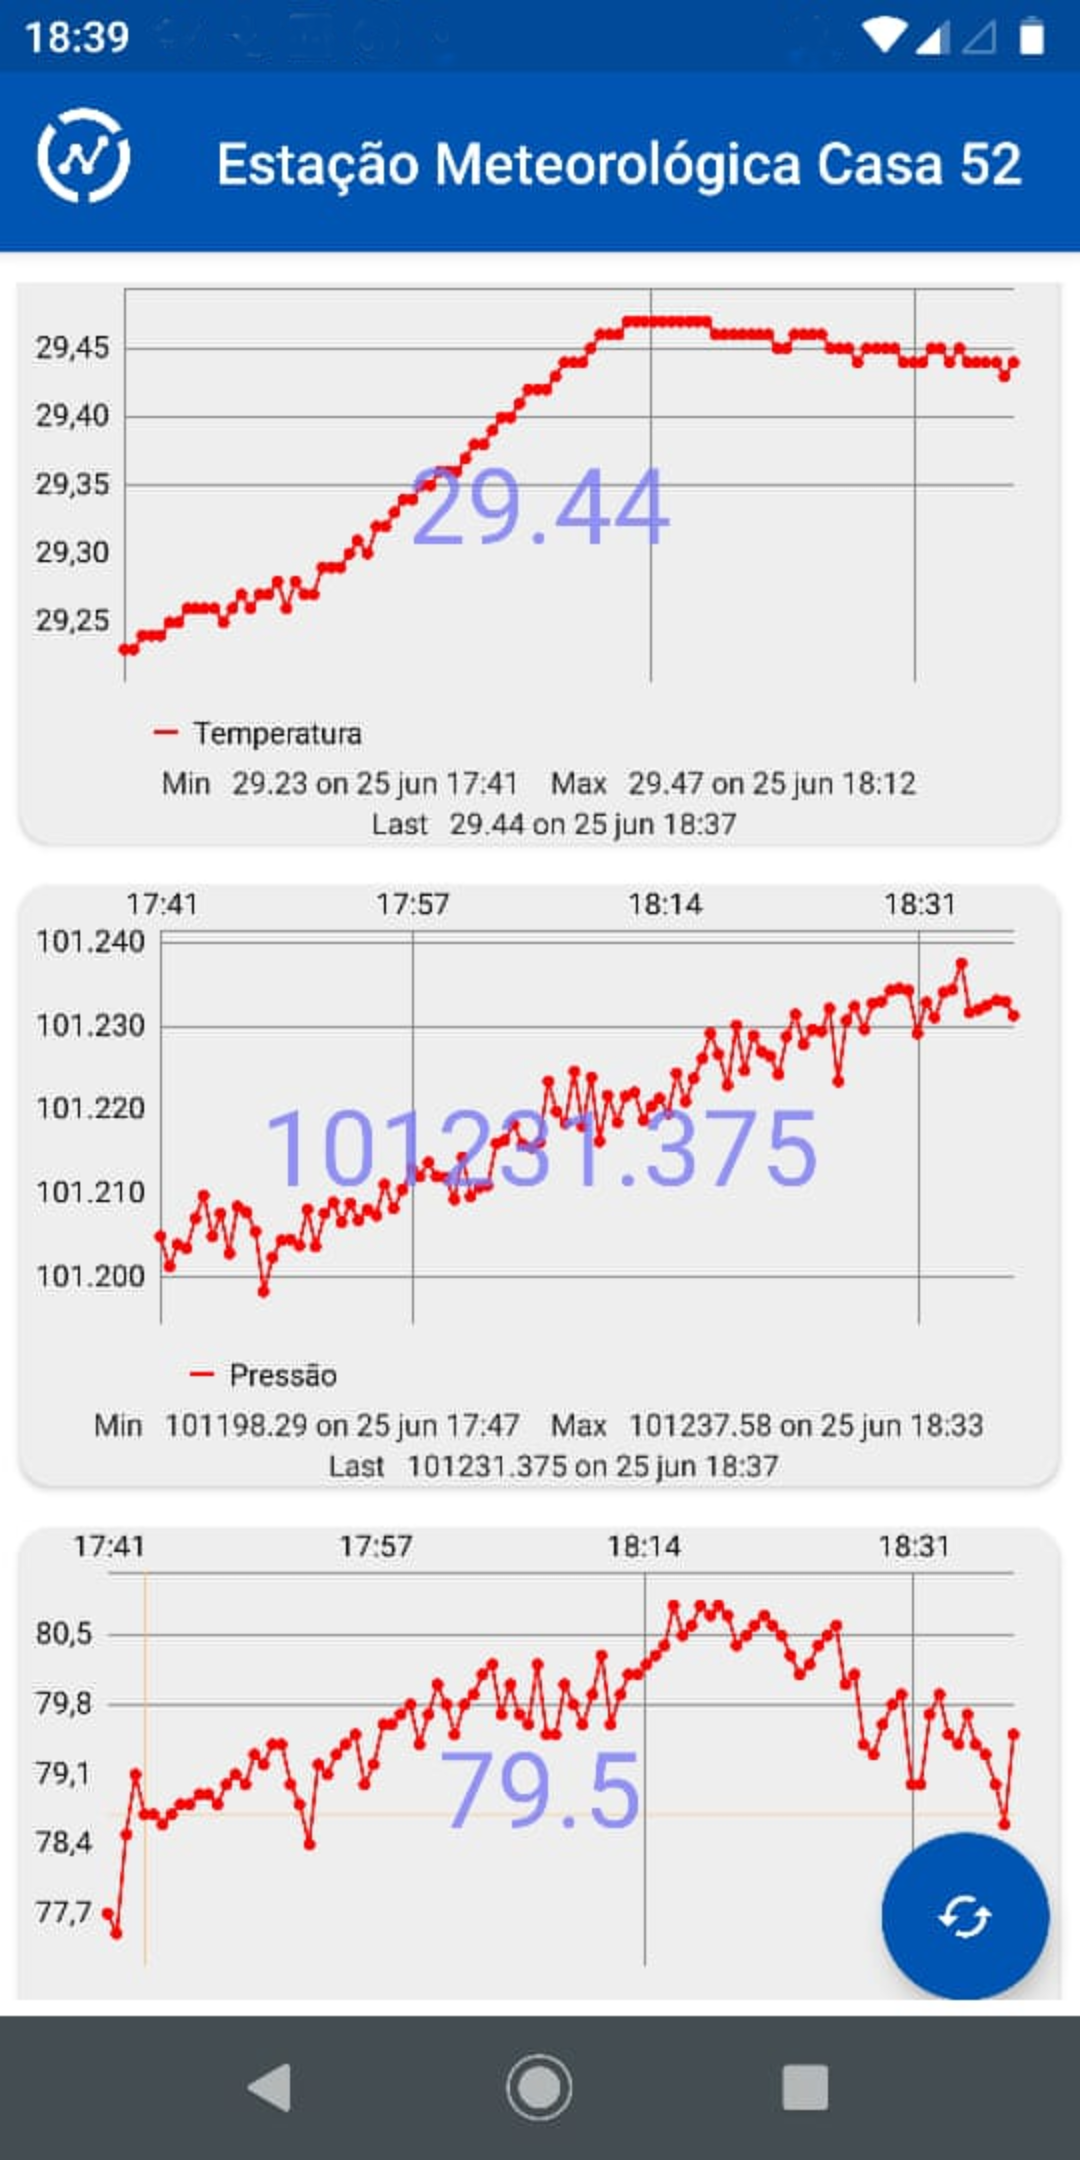
\includegraphics [scale=0.15]{Figuras/img_app.png}
    \legend{Fonte: ThingSpeak App }
    \label{fig:img_app}
\end{figure}

Depois de terminada a etapa de coleta dos dados pelo protótipo é preciso obter dados da plataforma REDEMET. Uma forma de fazer isso e com a API da própria plataforma que permite obter dados meteorológicos a cada hora do dia. No anexo \ref{scriptShell} contém o Shell Script fornecido da plataforma que permite realizar o trabalho de coleta. A plataforma ThingSpeak disponibilizará as informações da amostra do protótipo por meio de um arquivo no formato ".csv".

\subsection{Teste de hipótese}

As amostras coletadas têm tamanhos iguais são 90 observações para cada varíavel. Será utilizado um teste de igualdade entre médias para cada varíavel que consiste em cinco passos são eles:

\begin{enumerate}
   \item Formulação da Hipótese.
   \item Análise da distribuição amostral.
   \item Fixação da significância do teste.
   \item Cálculo da estatística-teste e verificação desse valor com as áreas de aceitação e rejeição do teste.
   \item Aceitação ou rejeição da hipótese.
\end{enumerate}

\subsubsection{Formulação da Hipótese}
As hipóteses serão comuns para todas as variáveis podendo ser definida como:

{\raggedright $\mu_1 \Rightarrow$ A média da variável em análise do protótipo. 
\newline $\mu_2 \Rightarrow$ A média da variável em análise da plataforma REDEMET. 
\newline $ H_0 \Rightarrow$ Hipótese nula.
\newline $ H_1 \Rightarrow$ Hipótese alternativa.

$
\begin{cases}
H_0: \mu_1 = \mu_2 \\
H_1: \mu_1 \neq \mu_1
\end{cases}
$
}

\subsubsection{Análise da distribuição amostral}

\setlength\parindent{2em} A análise da distribuição consiste em verificar se o comportamento das amostras para cada variável. Se segue o padrão da distribuição normal com a utilização de um teste de normalidade pelo módulo scipy.stats.normaltest. Confirmando esse fato será aplicado o teste de cauda superior. Caso uma das distribuições não seja normal será usado o teste estatístico de Wilcoxon. O teste será baseado no trabalho de \cite{d1973tests}. Basicamente o teste irá retornar uma variável chamada de p-valor que será comparado com o nível de significância.

\subsubsection{Fixação da significância do teste}

O nível de significância será o mesmo para todas as variáveis. Ele será utilizado para delimitar a área de aceitação e de rejeição da hipótese.

\begin{figure} [!h]
    \centering
    \caption{Delimitação da Área de rejeição em uma distribuição normal}
    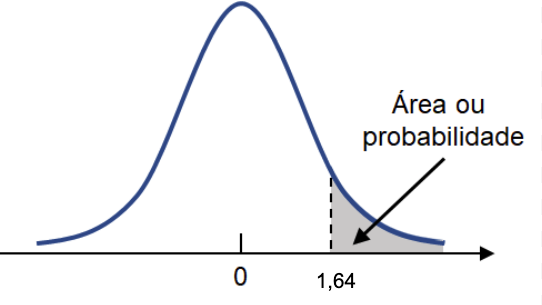
\includegraphics [scale=0.35]{Figuras/nivel_aceitacao.png}
    \legend{Fonte: Autor }
    \label{fig:img_distrNormal}
\end{figure}


\subsubsection{Cálculo da estatística teste e verificação desse valor com as áreas de aceitação e rejeição.}

Nessa etapa do teste aplica a fórmula, através da do módulo DescrStatsW, que tem como objetivo a comparação entre duas amostras para distribuições normais. Conforme fórmula abaixo.

\[\huge Z = \frac{(\bar{x_1} - \bar{x_2})-D_0}{\sqrt{\frac{s_1^2}{n_1} + \frac{s_2^2}{n_2}}}\]

{\raggedright $\bar{x_1} \Rightarrow$ A média da varíavel em análise do protótipo. 
\newline $\bar{x_2} \Rightarrow$ A média da varíavel em análise da plataforma REDEMET. 
\newline $D_0 \Rightarrow$ Diferença entre observações das amostras .
\newline $ s_1^2 \Rightarrow$ Variância da varíavel do protótipo.
\newline $ s_1^2 \Rightarrow$ Variância da varíavel da REDEMET.
\newline $ n_1 \Rightarrow$ número de observações da variável do protótipo.
\newline $ n_2 \Rightarrow$ número de observações da variável da REDEMET.
}

\setlength\parindent{2em}No caso da distribuição não ser classificada como normal será utilizada o módulo Wilcoxon para aplicar a seguinte estatística teste:

{\raggedright$$Z = \frac{T - \mu_T}{\sigma_T}$$

Onde:

$$\sigma_T = \sqrt{\frac{n(n + 1)(2n + 1)}{24}}$$
$$\mu_T = \frac{n(n+1)}{4}$$
$$T = min(R_1, R_2)$$

$ n \Rightarrow$ número de observações da variável do protótipo.
\newline $R_1$ = soma do ranking do grupo 1$n_1$
\newline $R_2$ = soma do ranking do grupo 2$n_2$
}

\subsubsection{Aceitação ou rejeição da hipótese}
\setlength\parindent{2em}
Na última etapa é feita uma comparação do valor encontrado no cálculo da estatística-teste e comparado com o nível de significância. No caso do intervalo de aceitação conter a estatística teste, aceita-se a hipótese nula como estatisticamente válida e rejeita-se a alternativa. Caso contrário é aceito a hipótese alternativa e rejeitado a nula.






\chapter{Resultados} \label{resultado}


Neste capítulo são apresentados, interpretados e analisados os resultados alcançados no trabalho. Será comparado as informações referentes ao custo do protótipo com as estações do mercado. Cada variável meteorológica será analisada com a exibição da sua distribuição por meio do gráfico de histograma, as estatísticas descritivas através de tabela, gráfico de box plot e aplicado o teste de hipóteses nos resultados obtidos.

\section{Comparação de Custos}

Segundo \cite{torres2015aquisiccao} uma estação meteorológica construída a partir da plataforma arduino apresenta custo de 4\% do valor de uma estação convencional de mercado. Cabe uma observação, esse trabalho em questão utilizava apenas os sensores de umidade, luminosidade e temperatura isso no ano de 2015 o custo divulgado pelo autor foi de $R\$$ 193,00. No trabalho em questão foram utilizados mais sensores e os custos podem ser observados conforme tabela \ref{tab:custos}.

\begin{table}[!h]
\centering
\begin{tabular}{|l|c|}
\hline
\textbf{Sensor}       & \textbf{Preço} \\ \hline
DHT-22                & R\$ 23,66      \\ \hline
BMP280                & R\$ 16,90      \\ \hline
Sensor DV10 e SV10    & R\$ 257,99     \\ \hline
Protoboard/Fios       & R\$ 15,90      \\ \hline
Arduino UNO           & R\$ 42,00      \\ \hline
Frete de Equipamentos & R\$ 30,00      \\ \hline
Total                 & R\$ 386,45     \\ \hline
\end{tabular}
\caption{Custo Estação Meteorológica baixo Custo }
\label{tab:custos}
\end{table}

Conforme explicações no trabalho de \cite{ocampo2019entraves} ainda não existe nenhum tipo de regulamentação para certificar as estações de superfície por parte da aeronáutica. Por isso no mercado não iremos encontrar estações com algum tipo de selo comprovando a categoria de uma determinada estação nesse cenário utilizei de estações comerciais que podem ser adquiridas via WEB para fins de comparação.

\begin{table}[!h]
\centering
\begin{tabular}{|l|c|}
\hline
\textbf{Estação Meteorológica}                               & \textbf{Preço} \\ \hline
Estação Meteorológica Vantage Vue Davis (300 metros) - K6250 & R\$ 6250,00    \\ \hline
Estação Meteorológica Nexus - 35.1075                        & R\$ 1897,50    \\ \hline
Estação de Temperatura e Umidade Davis 6382         & R\$ 3900,00   \\ \hline
Estação Meteorológica Vantage Pro2 Davis (Cabo) - K6152C     & R\$ 9000,00    \\ \hline
\end{tabular}
\caption{Fonte: site Clima e ambiente https://www.climaeambiente.com.br/}
\label{tab:custos_estacoes}
\end{table}

Na tabela \ref{tab:custos_estacoes} foi escolhido apenas estações que tenha mensurações similares a estação desenvolvida no trabalho o único sensor adicional nelas é o pluviométrico. Existem outras estações, que medem luminosidade, índices de raio UV. Entretanto, não seria muito justo comparar equipamentos que não possuem capacidades similares. É possível notar que o custo do protótipo desenvolvido nesse trabalho e de no máximo 20\% do valor de uma estação comercial.
 

\section{Análise dos dados}


\subsection{Análise da variável de temperatura}

Podemos observar no gráfico de histograma \ref{fig:dist_temperatura} sobre a variável temperatura que as medições feitas pelo protótipo tiveram poucas variações em relação a da plataforma REDEMET. 

\begin{figure} [!h]
    \centering
    \caption{Distribuição da variável Temperatura}    
    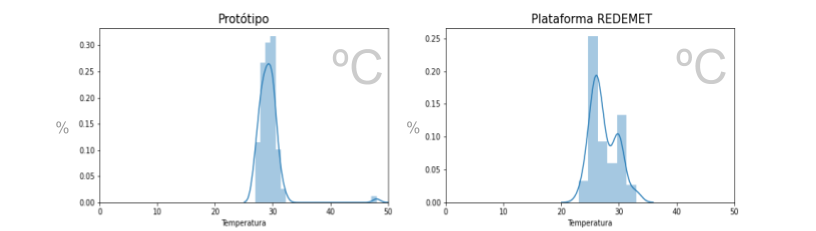
\includegraphics [scale = 0.5] {Figuras/dist_temp.png}
    \legend{Fonte: Gráfico elaborado pelo autor}
    \label{fig:dist_temperatura}
\end{figure}

É possível notar a presença de outliers nas medições feitas pelo protótipo. Facilmente observado no gráfico \ref{fig:box_temp}

\begin{figure} [!h]
    \centering
    \caption{Box Plot Temperatura}    
    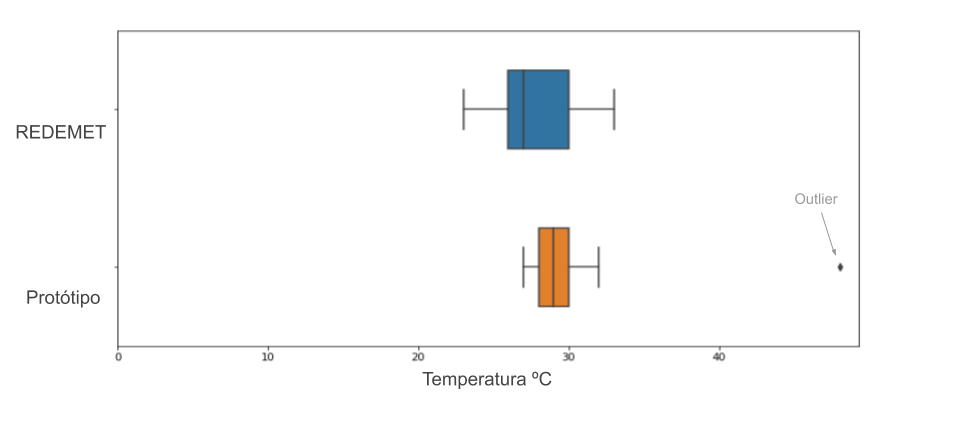
\includegraphics [scale = 0.45] {Figuras/box_temp.png}
    \legend{Fonte: Gráfico elaborado pelo autor}
    \label{fig:box_temp}
\end{figure}

Além de outliers é possível ver que a mediana das temperaturas coletadas pelo protótipo foi maior que a da plataforma REDEMET e que o menor valor de temperatura foi registrado na amostra da REDEMET. É o maior valor de temperatura foi registrado na amostra do protótipo justamente o outlier. Para confirmar essas observações e possível ver as estatísticas descritivas na tabela \ref{tab:est_desc_temp_prot}.

\begin{table}[!h]
\centering
\begin{tabular}{l|c|c|}
\cline{2-3}
                                                & \multicolumn{1}{l|}{\textbf{Temperatura REDEMET}} & \textbf{Temperatura Protótipo} \\ \hline
\multicolumn{1}{|l|}{Quantidade de Observações} & 90                                                & 90                             \\ \hline
\multicolumn{1}{|l|}{Média}                     & 27.37                                             & 29.30                          \\ \hline
\multicolumn{1}{|l|}{Desvio Padrão}             & 2.27                                              & 2.33                           \\ \hline
\multicolumn{1}{|l|}{Valor Mínimo}              & 23                                                & 27                             \\ \hline
\multicolumn{1}{|l|}{Valor Máximo}              & 33                                                & 48                             \\ \hline
\end{tabular}
\caption{Dados estatísticos variável temperatura}
\label{tab:est_desc_temp_prot}
\end{table}

\setlength\parindent{2em}
Aplicando o teste de distribuições o resultado foi que as amostras não são seguem o padrão da distribuição normal. Nesse caso será aplicado o cálculo estatístico de Wilcoxon, que deu como resultado que a hipótese H0 pode ser rejeitada com o pvalor de $4e-11$ um número muito próximo de zero. Nesse caso podemos concluir que para um nível de significância de 5\% as médias das temperaturas coletas pelo protótipo e pela plataforma REDEMET não são iguais.


\subsection{Análise da variável de pressão}

Na distribuição da variável de pressão podemos observar que ela foi mais uniforme e tivemos pouca diferença entre as amostras. Conforme gráfico \ref{fig:dist_pressao}

\begin{figure} [!h]
    \centering
    \caption{Distribuição da variável pressão}    
    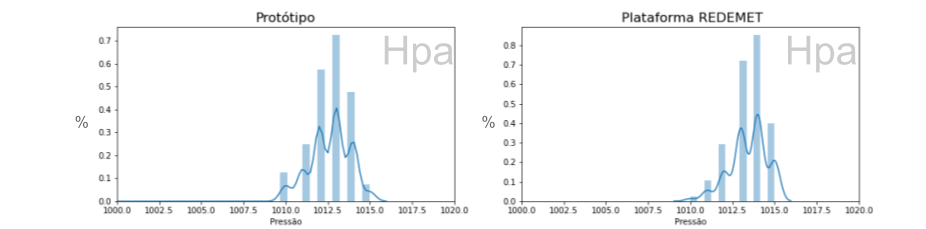
\includegraphics [scale = 0.5] {Figuras/dist_pressao.png}
    \label{fig:dist_pressao}
\end{figure}

Pelo gráfico \ref{fig:box_plot_pressao} é possível destacar a presença de outliers nas amostras. Visualmente as amostras têm resultados bem similares a diferença pode ser na questão de calibração do sensor. Nesse gráfico não é da para ver a mediana dos valores possivelmente foi igual algum intervalo interquartil do gráfico.

\begin{figure} [!h]
    \centering
    \caption{Box Plot Pressão}    
    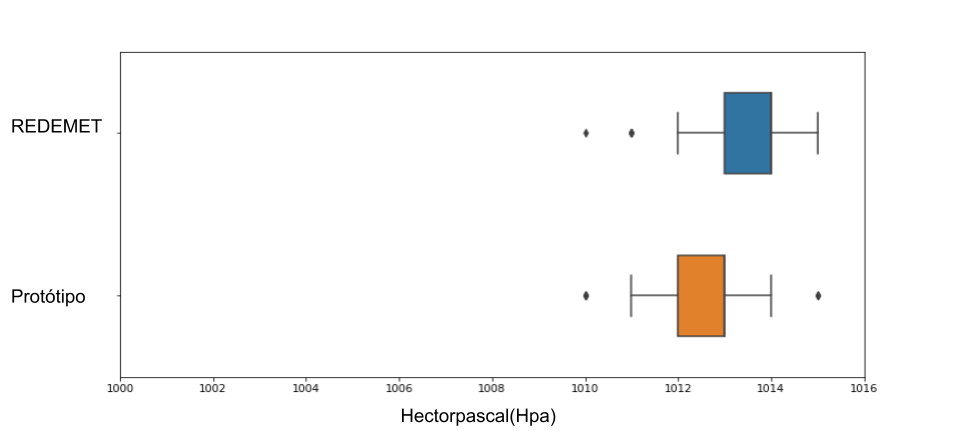
\includegraphics [scale = 0.45] {Figuras/box_plot_pressao.png}
    \label{fig:box_plot_pressao}
\end{figure}

Com as estatísticas descritivas da variável de pressão merece destaque o valor máximo que foi o mesmo para às duas amostras. O valor mínimo do protótipo é um outlier tivemos médias bem similares é um desvio padrão muito baixo na amostra da plataforma REDEMET. Conforme tabela \ref{tab:est_desc_pressao_prot}

\begin{table}[!h]
\centering
\begin{tabular}{l|c|c|}
\cline{2-3}
                                                & \multicolumn{1}{l|}{\textbf{Pressão REDEMET}} & \textbf{Pressão Protótipo} \\ \hline
\multicolumn{1}{|l|}{Quantidade de Observações} & 90                                            & 90                         \\ \hline
\multicolumn{1}{|l|}{Média}                     & 1013.44                                       & 1012.43                    \\ \hline
\multicolumn{1}{|l|}{Desvio Padrão}             & 1.11                                          & 2.2                        \\ \hline
\multicolumn{1}{|l|}{Valor Mínimo}              & 1010                                          & 995                        \\ \hline
\multicolumn{1}{|l|}{Valor Máximo}              & 1015                                          & 1015                       \\ \hline
\end{tabular}
\caption{Dados estatísticos variável pressão}
\label{tab:est_desc_pressao_prot}
\end{table}

O resultado do teste de normalidade foi favorável apenas para a amostra da plataforma REDEMET enquanto os dados do protótipo não se encaixaram em uma distribuição normal. Nesse caso será utilizado o cálculo estatístico de Wilcoxon que teve como resultado a rejeição da hipótese H0 com o pvalor muito baixo $1.73e-14$. Nesse caso podemos concluir que para um nível de significância de 5\% as médias das amostras coletas para a variável pressão do protótipo e da plataforma REDEMET não são iguais.

\subsection{Análise da variável de umidade}

As amostras da distribuição da variável de umidade são bem similares com poucas variações. Conforme gráfico \ref{fig:dist_umidade}. Visualmente pelo gráfico podemos notar que as destruições não seguem características de uma distribuição normal. Nenhum percentual de umidade foi registrado abaixo de 40\%. A maior parte das medições em ambas as amostras se concentrou próximas de 80\%.

\newpage

\begin{figure} [!h]
    \centering
    \caption{Distribuição da variável Umidade}
    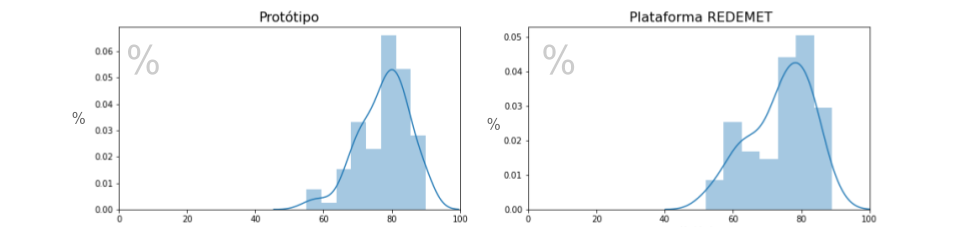
\includegraphics [scale = 0.5] {Figuras/dist_umidade.png}
    \label{fig:dist_umidade}
\end{figure}

Pelo gráfico \ref{fig:box_plot_umidade} podemos ver apenas um outlier na amostra do protótipo. A amostra do REDEMET tem mais variações nas medições do que a do protótipo. A mediana da amostra do protótipo é maior que a da amostra REDEMET. O maior valor de umidade foi registrado pela amostra do protótipo. O menor valor de umidade foi registrado pela plataforma REDEMET.

\begin{figure} [!h]
    \centering
    \caption{Box Plot Umidade}
    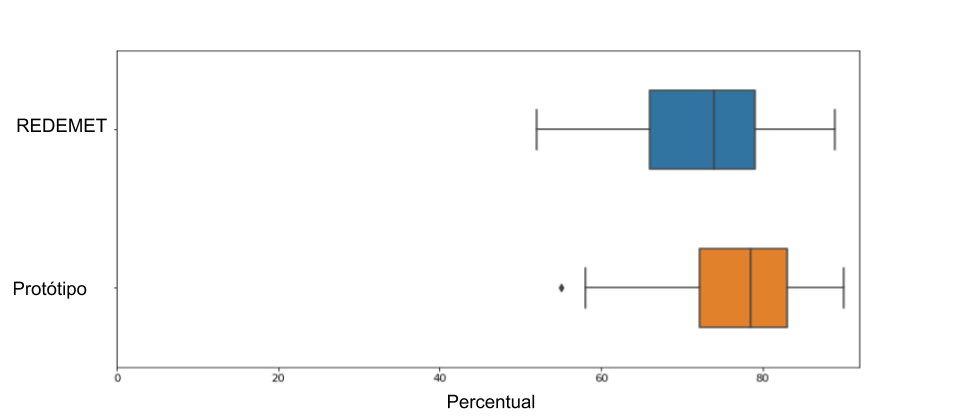
\includegraphics [scale = 0.5] {Figuras/box_plot_umidade.png}
    \label{fig:box_plot_umidade}
\end{figure}

Pela tabela \ref{tab:est_desc_umidade_prot} de dados estatísticos descritivos  podemos confirmar as observações feitas no gráfico. Podemos perceber um desvio padrão muito elevado nas amostras.

\begin{table}[!h]
\centering
\begin{tabular}{l|c|c|}
\cline{2-3}
                                                & \multicolumn{1}{l|}{\textbf{Umidade REDEMET}} & \textbf{Umidade Protótipo} \\ \hline
\multicolumn{1}{|l|}{Quantidade de Observações} & 90                                            & 90                         \\ \hline
\multicolumn{1}{|l|}{Média}                     & 73.84                                         & 77.67                      \\ \hline
\multicolumn{1}{|l|}{Desvio Padrão}             & 9.16                                          & 7.40                       \\ \hline
\multicolumn{1}{|l|}{Valor Mínimo}              & 52                                            & 55                         \\ \hline
\multicolumn{1}{|l|}{Valor Máximo}              & 89                                            & 90                         \\ \hline
\end{tabular}
\caption{Dados estatísticos variável umidade}
\label{tab:est_desc_umidade_prot}
\end{table}

Aplicando o teste de normalidade nas distribuições apenas a amostra da REDEMET pode ser classificada como normal. Aplicando o teste de Wilcoxon tivemos como resultado a rejeição da hipótese H0 com o pvalor muito baixo $2.94e-11$. Nesse caso podemos concluir que para um nível de significância de 5\% as médias das amostras coletas para a variável umidade não são iguais.

\subsection{Análise da variável direção do vento}

A distribuição das amostras para essa variável foi bem distinta. Como podemos observar no gráfico de distribuição. A concentração das medições ficou similar nas amostras com valores próximos a 100 graus.

\begin{figure} [!h]
    \centering
    \caption{Distribuição da variável direção do vento}    
    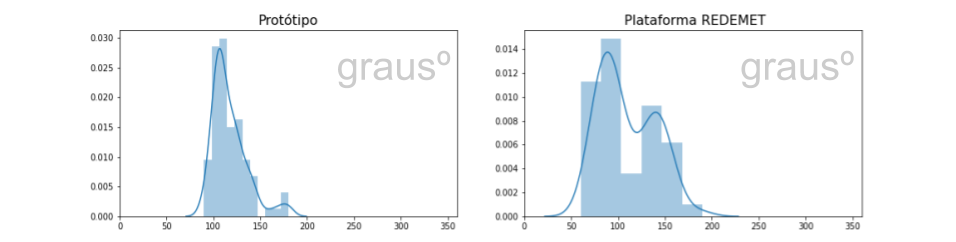
\includegraphics [scale = 0.5] {Figuras/dist_dirvento.png}
    \label{fig:dist_dirvento}
\end{figure}

No gráfico \ref{fig:box_plot_dirvento} existe a presença de outliers na amostra do protótipo. A mediana da amostra do protótipo foi superior a da REDEMET. Fica mais evidente a grande variação dos valores na amostra da plataforma REDEMET. 

\begin{figure} [!h]
    \centering
    \caption{Box Plot Direção do Vento}
    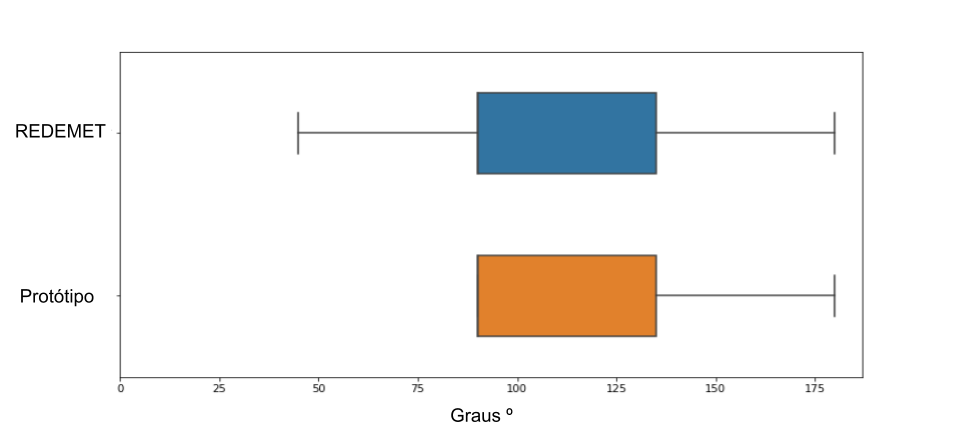
\includegraphics [scale = 0.5] {Figuras/box_plot_dirvento.png}
    \label{fig:box_plot_dirvento}
\end{figure}

Os valores de mensuração do sensor do protótipo são limitados aos pontos cardeais e colaterais o que dá no total oito valores (0º, 45º, 90º, 135º, 180º, 225º, 270º e 315º) possíveis enquanto os dados coletados na amostra REDEMET mostram maiores variações. As estatísticas descritivas mostram um grande desvio padrão na variável a média dos valores ficou bem próxima. Os valores máximo e mínimo mostram o problema de precisão do sensor do protótipo que não conseguiria medir o valor 60 nem 190.

\begin{table}[]
\centering
\begin{tabular}{l|c|c|}
\cline{2-3}
                                                & \multicolumn{1}{l|}{\textbf{Umidade REDEMET}} & \textbf{Umidade Protótipo} \\ \hline
\multicolumn{1}{|l|}{Quantidade de Observações} & 90                                            & 90                         \\ \hline
\multicolumn{1}{|l|}{Média}                     & 109.66                                        & 117.24                     \\ \hline
\multicolumn{1}{|l|}{Desvio Padrão}             & 29.65                                         & 18.82                      \\ \hline
\multicolumn{1}{|l|}{Valor Mínimo}              & 60                                            & 90                         \\ \hline
\multicolumn{1}{|l|}{Valor Máximo}              & 190                                           & 180                        \\ \hline
\end{tabular}
\caption{Dados estatísticos variável direção do vento}
\label{tab:est_desc_dirvento_prot}
\end{table}

No teste de normalidade o resultado foi que ambas as amostras não seguem o padrão da distribuição normal. Na aplicação do teste de Wilcoxon tivemos como resultado do pvalor de 0,00079 bem inferior ao nível de significância. Nesse caso podemos concluir que as médias das amostras do protótipo e da plataforma REDEMET não são iguais para um nível de significância de 5\%.

\subsection{Análise da variável velocidade do vento}

As mensurações de velocidade vento pelo protótipo não foram bem sucedidas houve a queima do sensor que conta as rotações das pás, o reed switch, durante os experimentos desse modo conforme o gráfico \ref{fig:dist_velvento} demonstra que a amostra do protótipo foram bem pequenas. 

\begin{figure} [!h]
    \centering
    \caption{Distribuição da variável direção do vento}    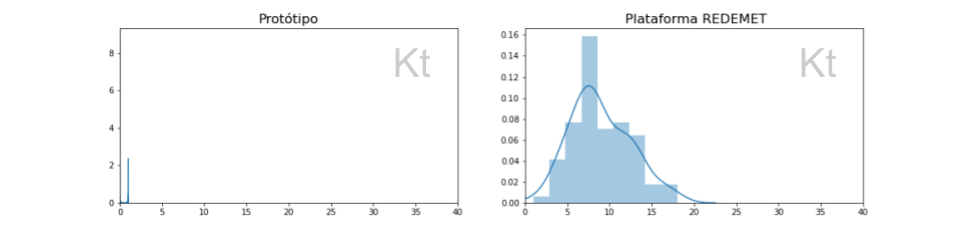
\includegraphics [scale = 0.5] {Figuras/dist_velvento.png}
    \label{fig:dist_velvento}
\end{figure}


Para confirmar que as mensurações de velocidade do vento não foram suficientes pelo protótipo no gráfico \ref{fig:box_plot_velvento} notamos que a amostra foi considerada como um outlier. Enquanto a amostra da plataforma REDEMET se mostrou bem distribuída e sem a presença de outliers. Com a média entre os valores de 25\% a 50\% da amostra. É com valor máximo superior a 17,5 kt e valor mínimo próximo à média dos valores coletados pelo protótipo.

\begin{figure} [!h]
    \centering
    \caption{Box Plot Velocidade do Vento}
    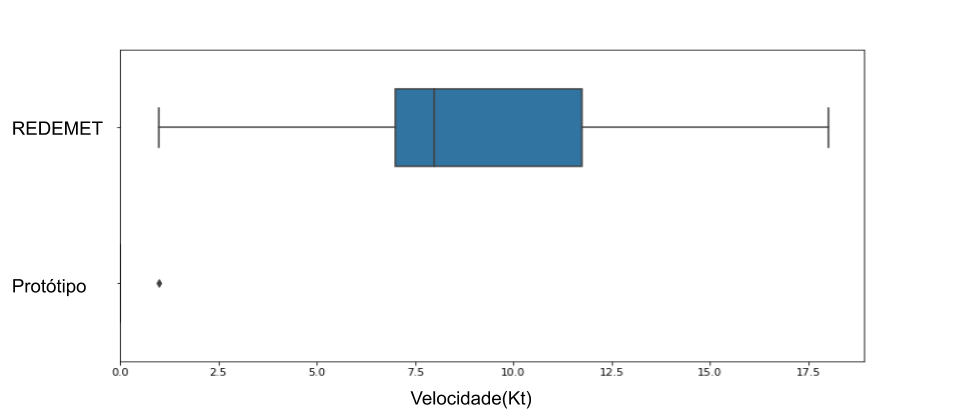
\includegraphics [scale = 0.5] {Figuras/box_plot_vento.png}
    \label{fig:box_plot_velvento}
\end{figure}

Observando os valores das estatísticas descritivas na tabela \ref{tab:est_desc_velvento_prot} se confirma as observações feitas na análise do gráfico de box plot.

\begin{table}[]
\centering
\begin{tabular}{l|c|c|}
\cline{2-3}
                                                & \multicolumn{1}{l|}{\textbf{Umidade REDEMET}} & \textbf{Umidade Protótipo} \\ \hline
\multicolumn{1}{|l|}{Quantidade de Observações} & 90                                            & 90                         \\ \hline
\multicolumn{1}{|l|}{Média}                     & 8.94                                          & 0.011                      \\ \hline
\multicolumn{1}{|l|}{Desvio Padrão}             & 3.56                                          & 0.01                       \\ \hline
\multicolumn{1}{|l|}{Valor Mínimo}              & 1                                             & 0                          \\ \hline
\multicolumn{1}{|l|}{Valor Máximo}              & 18                                            & 1                          \\ \hline
\end{tabular}
\caption{Dados estatísticos variável velocidade do vento}
\label{tab:est_desc_velvento_prot}
\end{table}

É evidente que a distribuição do protótipo não é normal aplicando o teste de normalidade essa observação se confirmou e a distribuição da REDEMET foi classificada como normal. Foi aplicado o teste de Wilcoxon mesmo já sabendo que o resultado seria rejeição que se confirmou com um pvalor de 0,0014. É possível concluir que as médias das amostras do protótipo e da plataforma REDEMET não são iguais para um nível de significância de 5\%.


\chapter{Conclusão} \label{conclusao} 

No Brasil, alguns aeroportos regionais não possuem acessos a dados de meteorológica para tomada de decisões por meio da plataforma REDEMET. Uma alternativa para esses aeroportos seriam a obtenção de dados meteorológicos com o uso de estação meteorológica própria que muitas das vezes tem um custo considerável para a categoria regional de aeroportos. Esse trabalho elaborou um protótipo de estações meteorológica com a utilização de sensores da plataforma arduino, a disponibilização e armazenamento dos dados em tempo real através da plataforma de nuvem Thingspeak com objetivo de baratear custos e fornecer dados adequados para os aeroportos regionais. O trabalho coletou amostras da plataforma REDEMET e do protótipo, verificou qual o tipo de distribuição os se enquadram para a aplicação de teste estatístico adequado. No trabalho foi utilizado o teste de Wilcoxon para verificar se as médias das variáveis nas amostras poderiam ser consideradas iguais com um nível de significância de 5\%.

Na comparação feita o resultado foi de não igualdade entre as médias dos dados coletados para um nível de significância de 5\% em nenhuma variável meteorológica. Com o destaque negativo para as amostras coletadas pelo sensor de vento(SV10) que queimou durante o experimento. De forma que não se mostra verdadeira a hipótese do trabalho.

Esses resultados demonstram que não podemos utilizar os dados coletados pelo protótipo para observações locais que ocorrem no caso de incidentes ou acidentes aeronáuticos. É possível utilizar para observações regulares desde que fatores como posição e calibração do sensor esteja devidamente ajustado que podem ter contribuido para que a hipótese fosse rejeitada.

Sobre o fator localização é fato que o protótipo não está no mesmo local que estação da REDEMET então pode não capturar as mesmas condições meteorológicas. Entretanto, as variações de temperatura e pressão, por exemplo, na região metropolitana de Fortaleza onde o experimento foi realizado são pequenas. A calibração dos sensores não ser a mesma da plataforma REDE pode ter sido o grande fator a se considerar visto que o trabalho utilizou os dispositivos conforme a configuração de fábrica sem nenhum tipo de calibração.


%%====== Section ========%
\section{Trabalhos Futuros}\label{trabalhosFuturos}

Esse trabalho não considerou utilizar modelos matemáticos para a calibração de sensores para trabalhos futuros seria proveitoso avaliar as mensurações sem e com calibração. Provando ou não possíveis diferenças entre as medições. Outro fator muito importante seria realizar o experimento dentro de sítio aeroportuário de uma aeroporto regional atendido pela plataforma REDEMET, desse modo, a localização da estação teria pouca interferência. Por fim utilizar outros sensores compatíveis com a plataforma arduino para teste especialmente para medição da direção e velocidade do vento.




%% -------------- Elementos Pós-Textuais -----------------%%
\postextual  
\bibliography{bibliografia} % Referências bibliográficas
%-------------------------------------------------------------
%---------------------- Apêndices ----------------------------
%-------------------------------------------------------------

\begin{apendicesenv}
\partapendices  % Indica o início dos Apendices


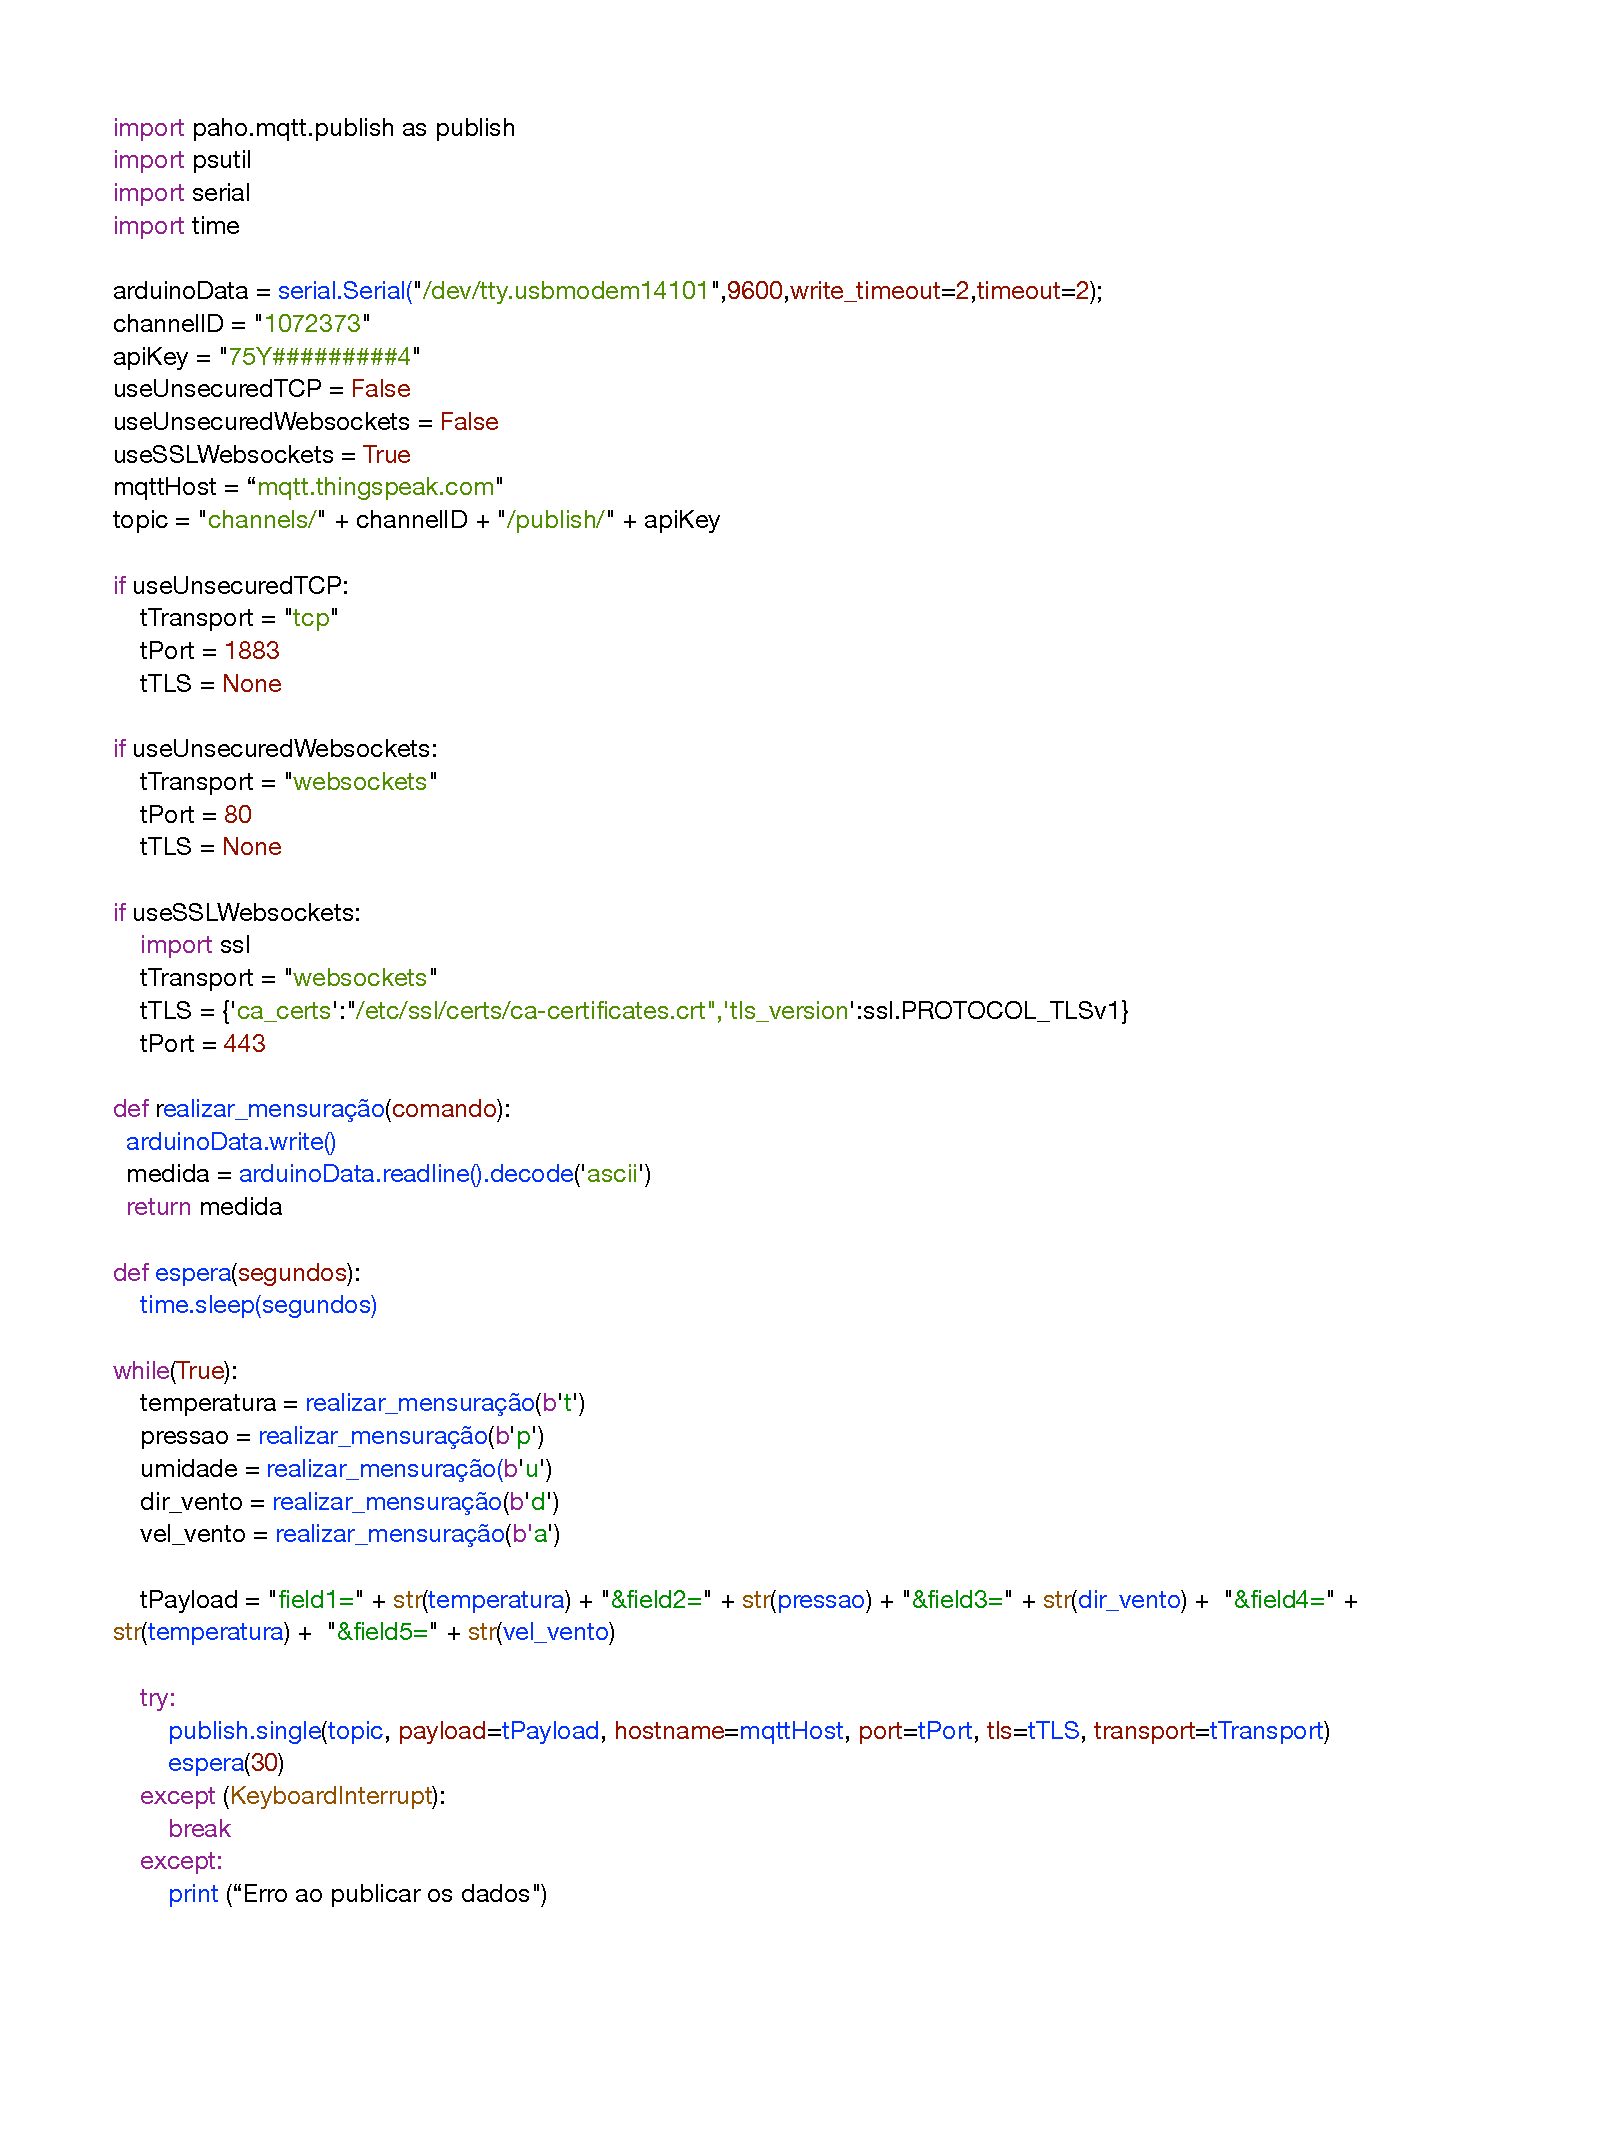
\includepdf[scale=0.85,pages=1,pagecommand=\chapter{Código Python}\label{PythonScript}]{Arq_Pdf/Script_Python.pdf}


%I2C Scanner
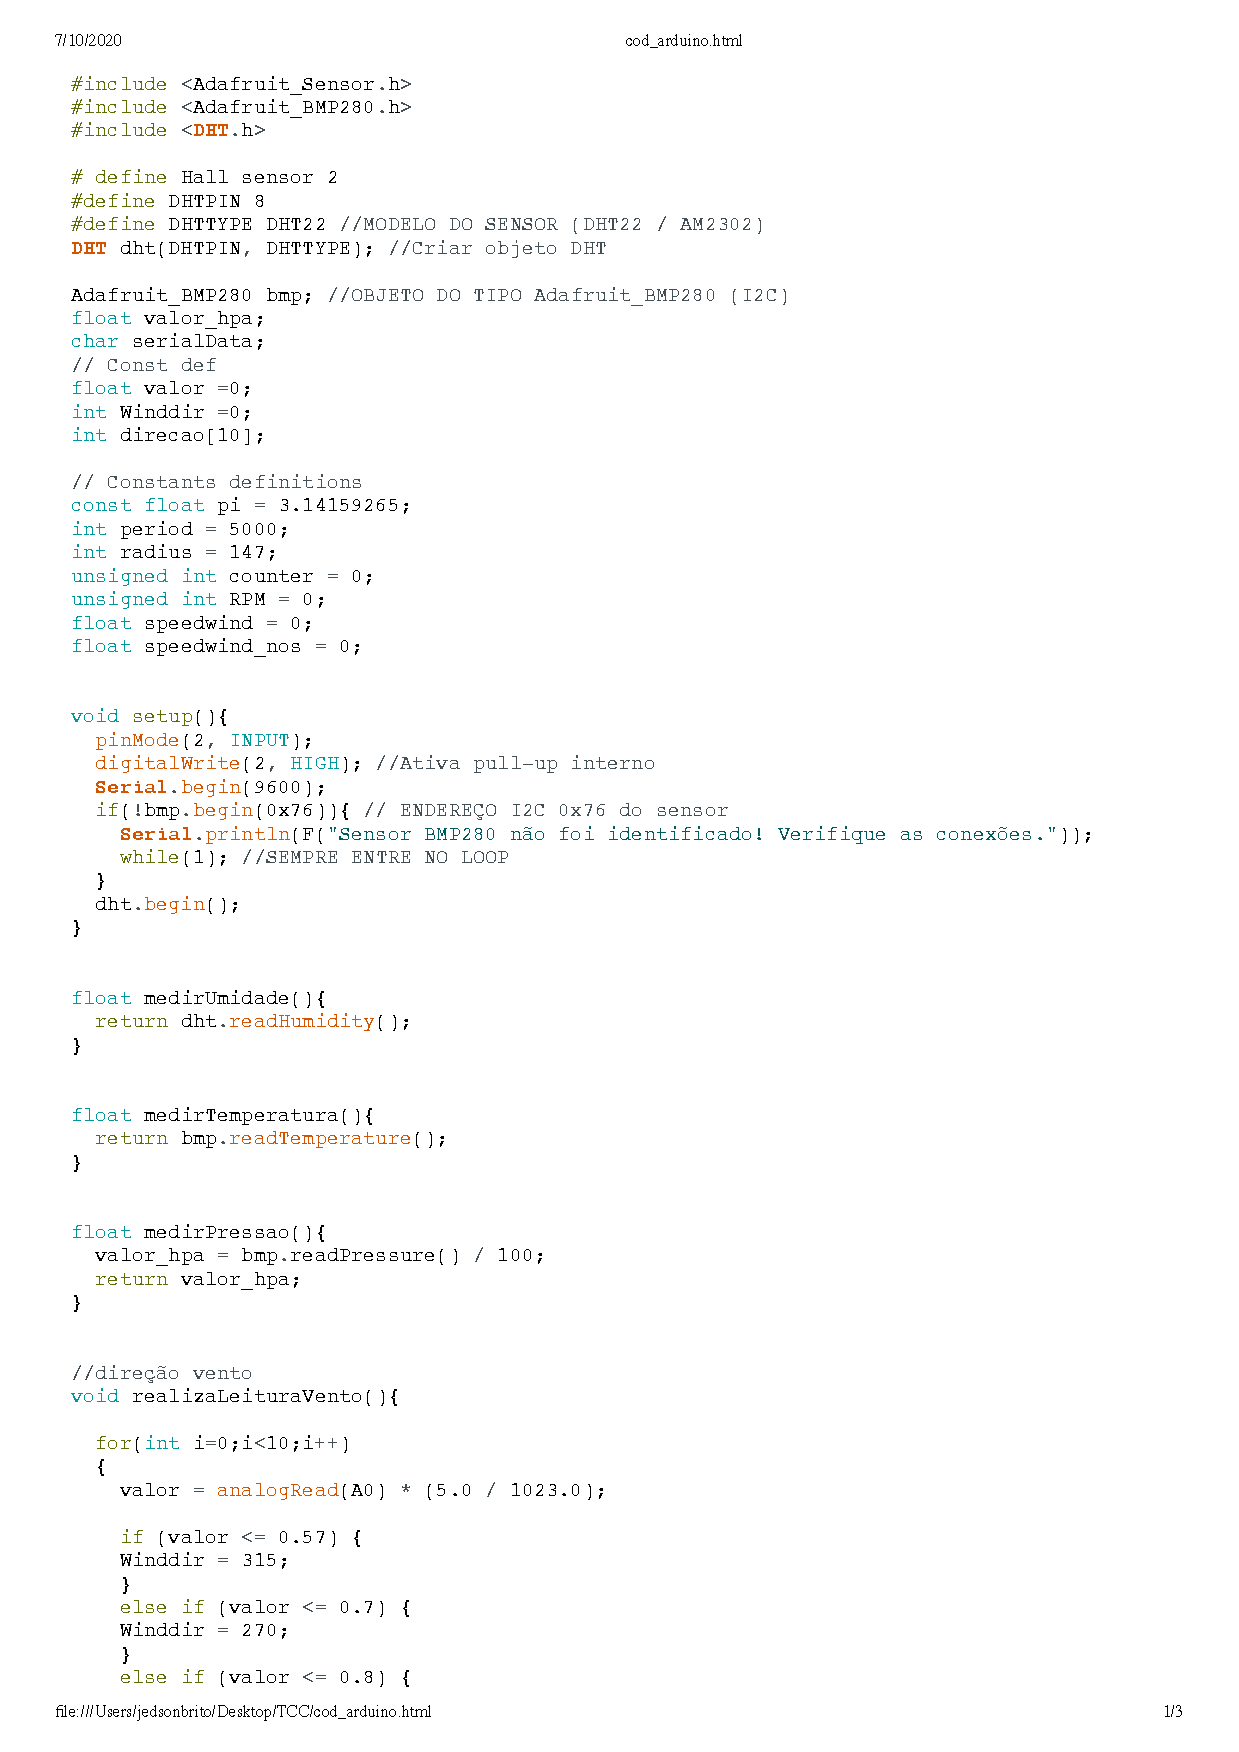
\includepdf[scale=0.75,pages=1,pagecommand=\chapter{Código Arduíno IDE}\label{CodigoArd}]{Arq_Pdf/cod_arduino.pdf}

\includepdf[scale=0.85,pages={2-3}]{Arq_Pdf/cod_arduino.pdf}

%Os apêndices devem ser identificados por letras maiúsculas consecutivas (APÊNDICE A, APÊNDICE B, etc), travessão e os respectivos títulos, devendo estar centralizados na folha. 

\end{apendicesenv}

%----------------------------------------------------------------
%---------------------- Anexos ----------------------------------
%----------------------------------------------------------------

\begin{anexosenv}
\partanexos   % indica o início dos anexos


%Manual Anemometro
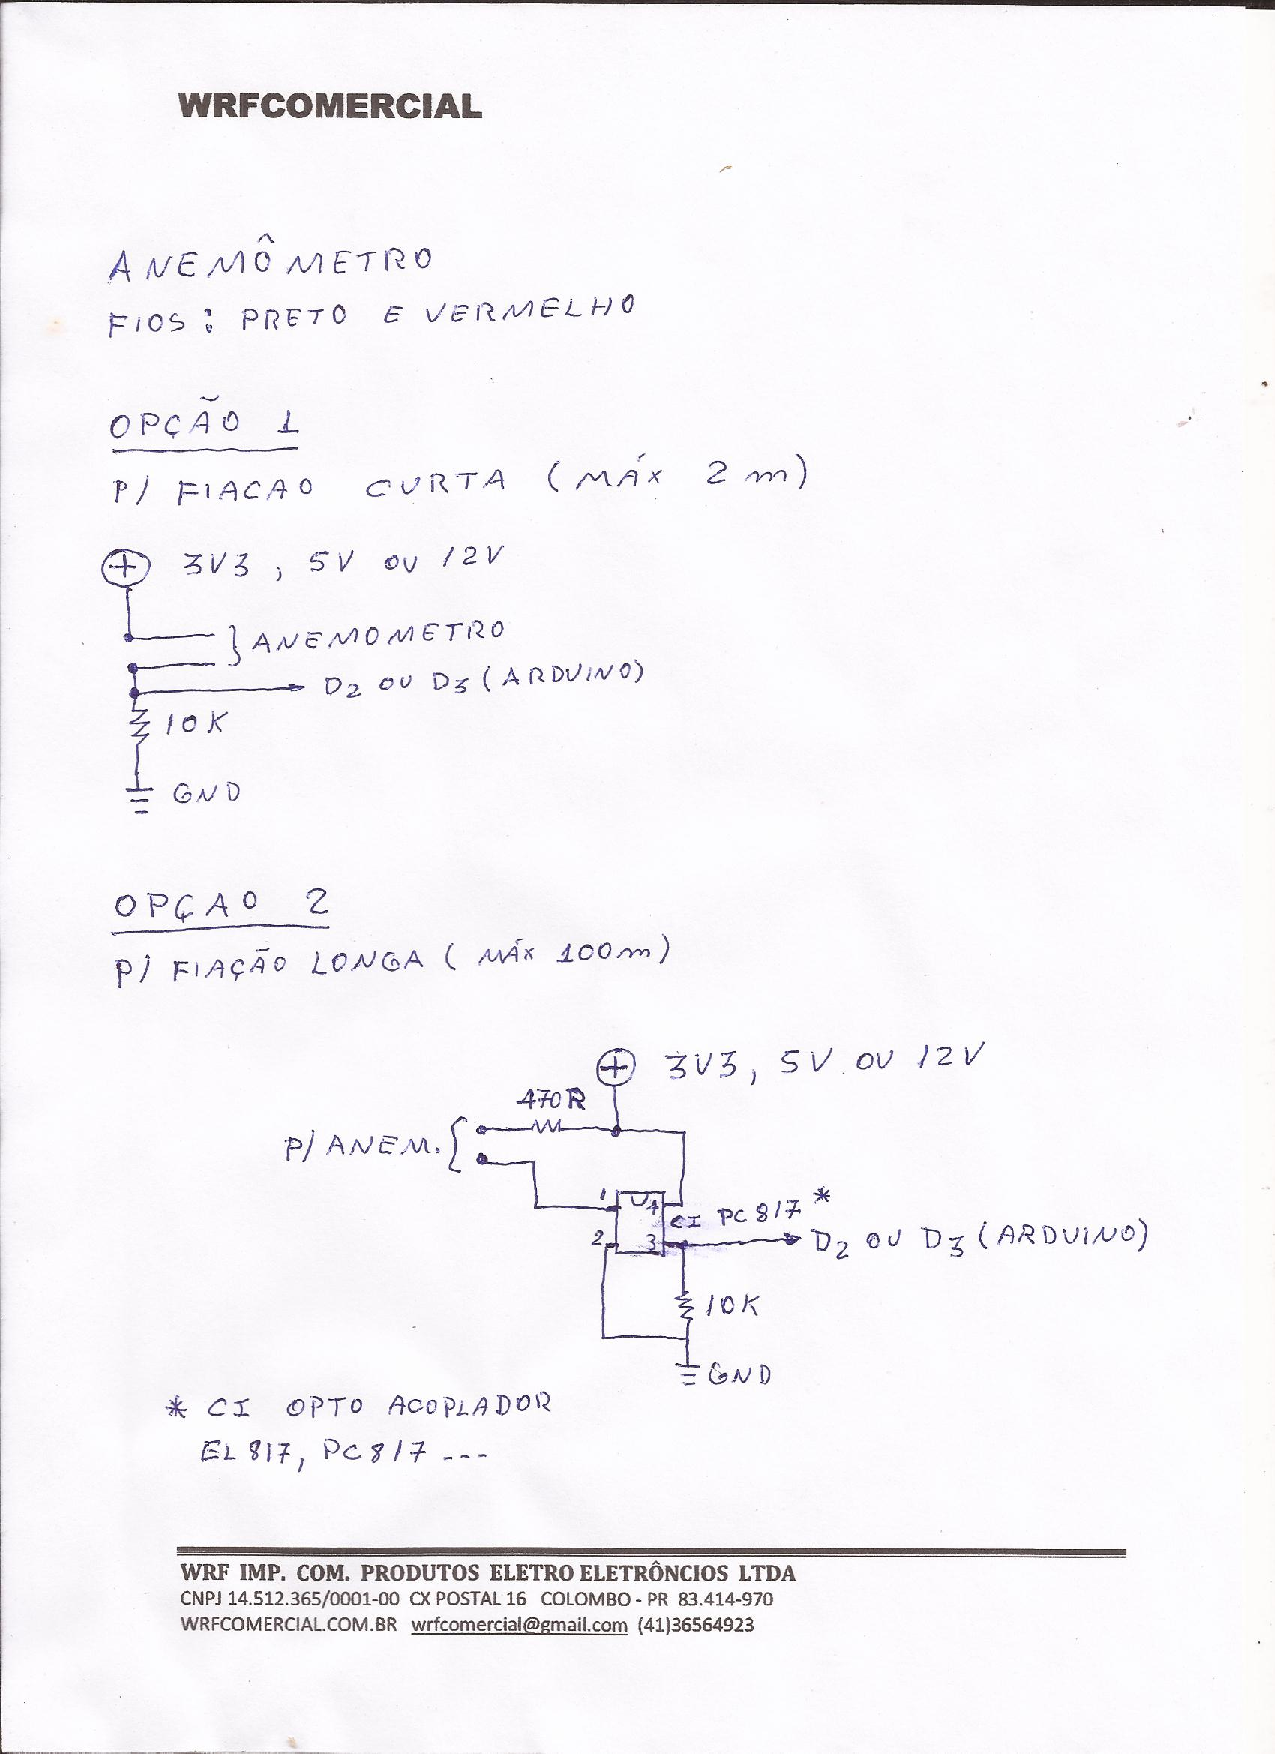
\includepdf[scale=0.65,pages=1,pagecommand=\chapter{Manual Anemômetro Fabricante WRF}\label{manAnemot}]{Arq_Pdf/AnemDrive1.pdf}

%Manual Anemografo
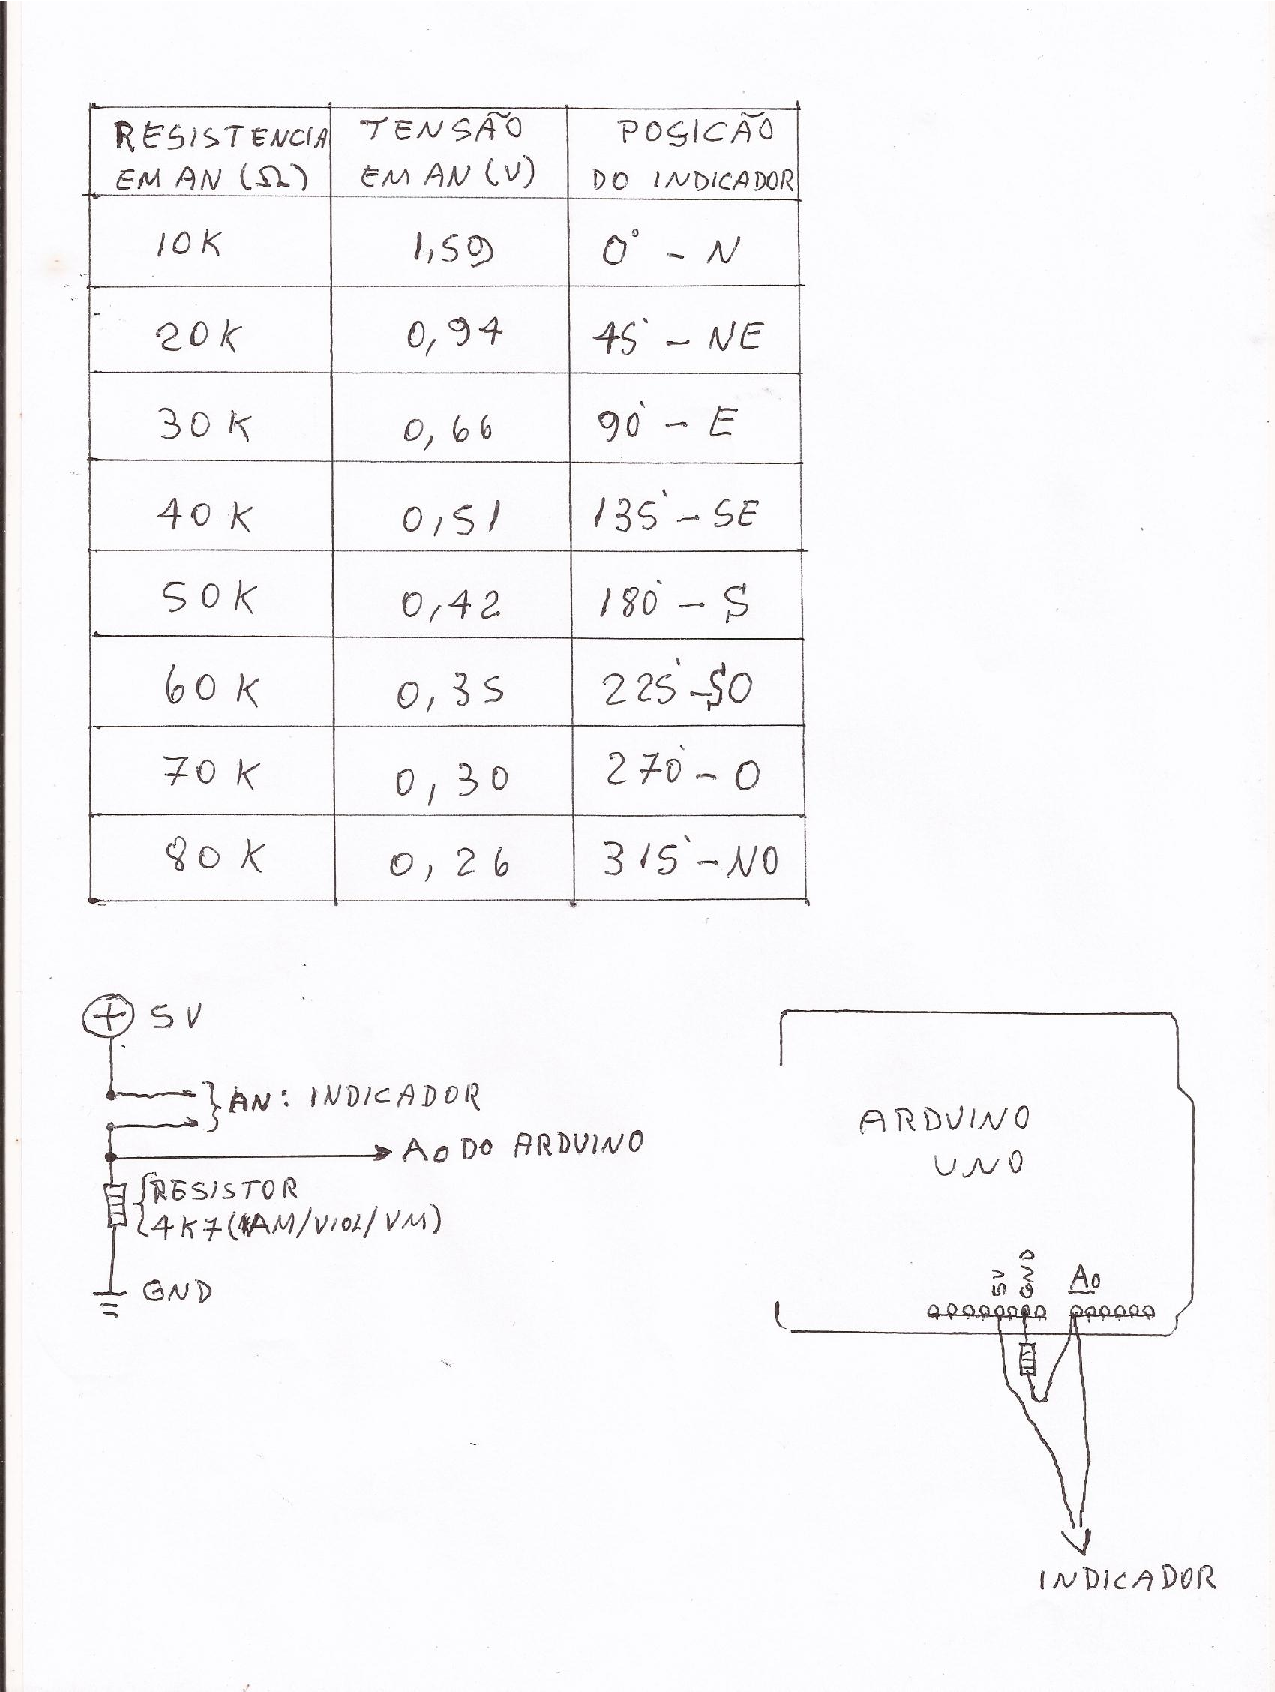
\includepdf[scale=0.65,pages=1,pagecommand=\chapter{Manual Biruta Fabricante WRF}\label{manAnemog}]{Arq_Pdf/BirutaTabela.pdf}

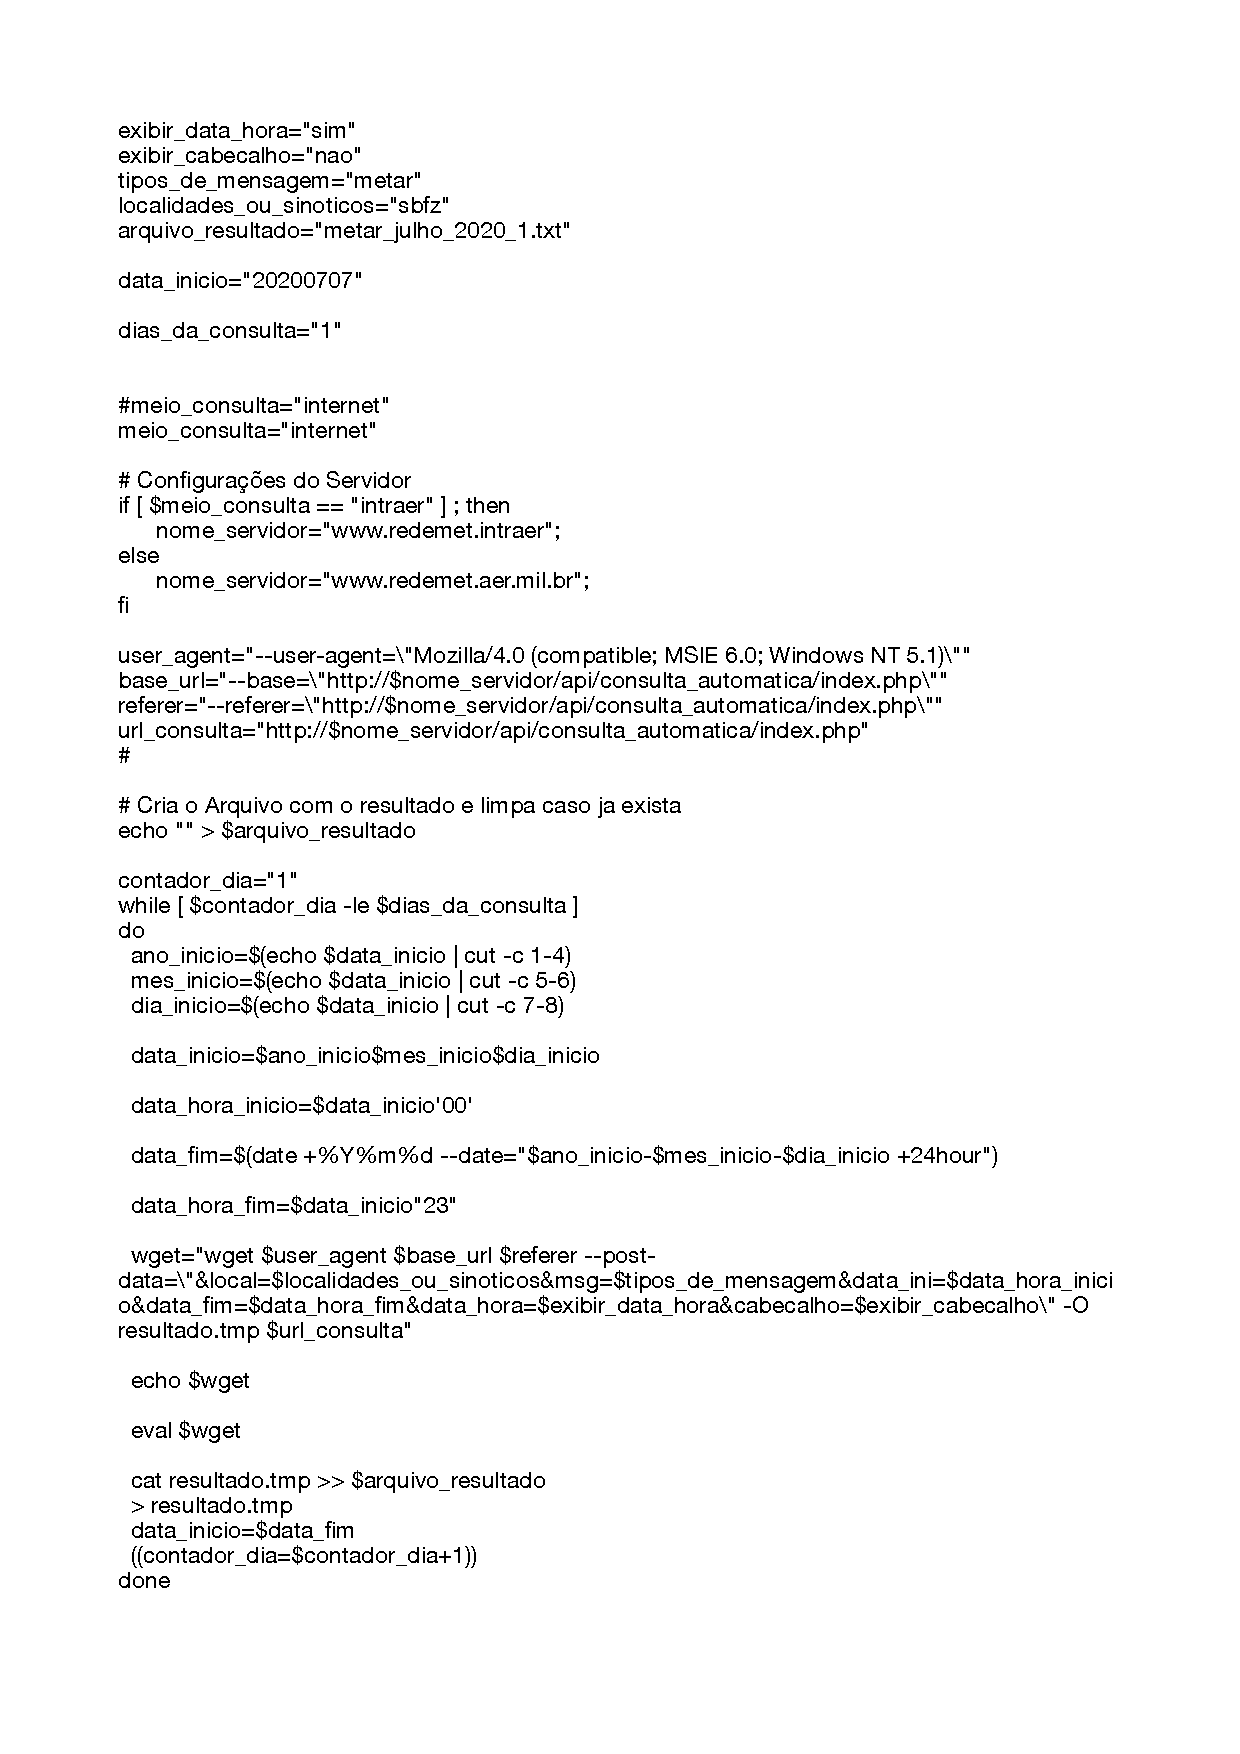
\includepdf[scale=0.85,pages=1,pagecommand=\chapter{Shell Script Redemet}\label{scriptShell}]{Arq_Pdf/shellScript_redemet.pdf}



\end{anexosenv}

\phantompart  \printindex  % Índice Remissivo
% ----------------------------------------------------------
\end{document}  % fim do documento

